\documentclass[aspectratio=169]{beamer}
\usetheme[
  block=fill,
  background=light,
  titleformat=smallcaps,
  progressbar=frametitle,
  numbering=none,
]{metropolis}
\setbeamersize{text margin left=.5cm,text margin right=.5cm}

%%%%%%%%%%%%%%%%%%%%%%%%%%%%%%%%%%%%%%%%%%
%% Packages
%%%%%%%%%%%%%%%%%%%%%%%%%%%%%%%%%%%%%%%%%%

% Tikz
\usepackage{tikz}
\usetikzlibrary{chains,arrows,automata,fit,positioning,calc}

% Colors
\usepackage{xcolor}

% Images
\usepackage{graphics}
\graphicspath{{img/}}

% Math Symbols
\usepackage{stmaryrd}

%%%%%%%%%%%%%%%%%%%%%%%%%%%%%%%%%%%%%%%%%%
%% Macros
%%%%%%%%%%%%%%%%%%%%%%%%%%%%%%%%%%%%%%%%%%
\renewcommand\alert[1]{\textcolor{mLightBrown}{#1}}

%%%%%%%%%%%%%%%%%%%%%%%%%%%%%%%%%%%%%%%%%%
%% Agda imports
%%%%%%%%%%%%%%%%%%%%%%%%%%%%%%%%%%%%%%%%%%

%% ODER: format ==         = "\mathrel{==}"
%% ODER: format /=         = "\neq "
%
%
\makeatletter
\@ifundefined{lhs2tex.lhs2tex.sty.read}%
  {\@namedef{lhs2tex.lhs2tex.sty.read}{}%
   \newcommand\SkipToFmtEnd{}%
   \newcommand\EndFmtInput{}%
   \long\def\SkipToFmtEnd#1\EndFmtInput{}%
  }\SkipToFmtEnd

\newcommand\ReadOnlyOnce[1]{\@ifundefined{#1}{\@namedef{#1}{}}\SkipToFmtEnd}
\usepackage{amstext}
\usepackage{amssymb}
\usepackage{stmaryrd}
\DeclareFontFamily{OT1}{cmtex}{}
\DeclareFontShape{OT1}{cmtex}{m}{n}
  {<5><6><7><8>cmtex8
   <9>cmtex9
   <10><10.95><12><14.4><17.28><20.74><24.88>cmtex10}{}
\DeclareFontShape{OT1}{cmtex}{m}{it}
  {<-> ssub * cmtt/m/it}{}
\newcommand{\texfamily}{\fontfamily{cmtex}\selectfont}
\DeclareFontShape{OT1}{cmtt}{bx}{n}
  {<5><6><7><8>cmtt8
   <9>cmbtt9
   <10><10.95><12><14.4><17.28><20.74><24.88>cmbtt10}{}
\DeclareFontShape{OT1}{cmtex}{bx}{n}
  {<-> ssub * cmtt/bx/n}{}
\newcommand{\tex}[1]{\text{\texfamily#1}}	% NEU

\newcommand{\Sp}{\hskip.33334em\relax}


\newcommand{\Conid}[1]{\mathit{#1}}
\newcommand{\Varid}[1]{\mathit{#1}}
\newcommand{\anonymous}{\kern0.06em \vbox{\hrule\@width.5em}}
\newcommand{\plus}{\mathbin{+\!\!\!+}}
\newcommand{\bind}{\mathbin{>\!\!\!>\mkern-6.7mu=}}
\newcommand{\rbind}{\mathbin{=\mkern-6.7mu<\!\!\!<}}% suggested by Neil Mitchell
\newcommand{\sequ}{\mathbin{>\!\!\!>}}
\renewcommand{\leq}{\leqslant}
\renewcommand{\geq}{\geqslant}
\usepackage{polytable}

%mathindent has to be defined
\@ifundefined{mathindent}%
  {\newdimen\mathindent\mathindent\leftmargini}%
  {}%

\def\resethooks{%
  \global\let\SaveRestoreHook\empty
  \global\let\ColumnHook\empty}
\newcommand*{\savecolumns}[1][default]%
  {\g@addto@macro\SaveRestoreHook{\savecolumns[#1]}}
\newcommand*{\restorecolumns}[1][default]%
  {\g@addto@macro\SaveRestoreHook{\restorecolumns[#1]}}
\newcommand*{\aligncolumn}[2]%
  {\g@addto@macro\ColumnHook{\column{#1}{#2}}}

\resethooks

\newcommand{\onelinecommentchars}{\quad-{}- }
\newcommand{\commentbeginchars}{\enskip\{-}
\newcommand{\commentendchars}{-\}\enskip}

\newcommand{\visiblecomments}{%
  \let\onelinecomment=\onelinecommentchars
  \let\commentbegin=\commentbeginchars
  \let\commentend=\commentendchars}

\newcommand{\invisiblecomments}{%
  \let\onelinecomment=\empty
  \let\commentbegin=\empty
  \let\commentend=\empty}

\visiblecomments

\newlength{\blanklineskip}
\setlength{\blanklineskip}{0.66084ex}

\newcommand{\hsindent}[1]{\quad}% default is fixed indentation
\let\hspre\empty
\let\hspost\empty
\newcommand{\NB}{\textbf{NB}}
\newcommand{\Todo}[1]{$\langle$\textbf{To do:}~#1$\rangle$}

\EndFmtInput
\makeatother
%
%
%
%
%
%
% This package provides two environments suitable to take the place
% of hscode, called "plainhscode" and "arrayhscode". 
%
% The plain environment surrounds each code block by vertical space,
% and it uses \abovedisplayskip and \belowdisplayskip to get spacing
% similar to formulas. Note that if these dimensions are changed,
% the spacing around displayed math formulas changes as well.
% All code is indented using \leftskip.
%
% Changed 19.08.2004 to reflect changes in colorcode. Should work with
% CodeGroup.sty.
%
\ReadOnlyOnce{polycode.fmt}%
\makeatletter

\newcommand{\hsnewpar}[1]%
  {{\parskip=0pt\parindent=0pt\par\vskip #1\noindent}}

% can be used, for instance, to redefine the code size, by setting the
% command to \small or something alike
\newcommand{\hscodestyle}{}

% The command \sethscode can be used to switch the code formatting
% behaviour by mapping the hscode environment in the subst directive
% to a new LaTeX environment.

\newcommand{\sethscode}[1]%
  {\expandafter\let\expandafter\hscode\csname #1\endcsname
   \expandafter\let\expandafter\endhscode\csname end#1\endcsname}

% "compatibility" mode restores the non-polycode.fmt layout.

\newenvironment{compathscode}%
  {\par\noindent
   \advance\leftskip\mathindent
   \hscodestyle
   \let\\=\@normalcr
   \let\hspre\(\let\hspost\)%
   \pboxed}%
  {\endpboxed\)%
   \par\noindent
   \ignorespacesafterend}

\newcommand{\compaths}{\sethscode{compathscode}}

% "plain" mode is the proposed default.
% It should now work with \centering.
% This required some changes. The old version
% is still available for reference as oldplainhscode.

\newenvironment{plainhscode}%
  {\hsnewpar\abovedisplayskip
   \advance\leftskip\mathindent
   \hscodestyle
   \let\hspre\(\let\hspost\)%
   \pboxed}%
  {\endpboxed%
   \hsnewpar\belowdisplayskip
   \ignorespacesafterend}

\newenvironment{oldplainhscode}%
  {\hsnewpar\abovedisplayskip
   \advance\leftskip\mathindent
   \hscodestyle
   \let\\=\@normalcr
   \(\pboxed}%
  {\endpboxed\)%
   \hsnewpar\belowdisplayskip
   \ignorespacesafterend}

% Here, we make plainhscode the default environment.

\newcommand{\plainhs}{\sethscode{plainhscode}}
\newcommand{\oldplainhs}{\sethscode{oldplainhscode}}
\plainhs

% The arrayhscode is like plain, but makes use of polytable's
% parray environment which disallows page breaks in code blocks.

\newenvironment{arrayhscode}%
  {\hsnewpar\abovedisplayskip
   \advance\leftskip\mathindent
   \hscodestyle
   \let\\=\@normalcr
   \(\parray}%
  {\endparray\)%
   \hsnewpar\belowdisplayskip
   \ignorespacesafterend}

\newcommand{\arrayhs}{\sethscode{arrayhscode}}

% The mathhscode environment also makes use of polytable's parray 
% environment. It is supposed to be used only inside math mode 
% (I used it to typeset the type rules in my thesis).

\newenvironment{mathhscode}%
  {\parray}{\endparray}

\newcommand{\mathhs}{\sethscode{mathhscode}}

% texths is similar to mathhs, but works in text mode.

\newenvironment{texthscode}%
  {\(\parray}{\endparray\)}

\newcommand{\texths}{\sethscode{texthscode}}

% The framed environment places code in a framed box.

\def\codeframewidth{\arrayrulewidth}
\RequirePackage{calc}

\newenvironment{framedhscode}%
  {\parskip=\abovedisplayskip\par\noindent
   \hscodestyle
   \arrayrulewidth=\codeframewidth
   \tabular{@{}|p{\linewidth-2\arraycolsep-2\arrayrulewidth-2pt}|@{}}%
   \hline\framedhslinecorrect\\{-1.5ex}%
   \let\endoflinesave=\\
   \let\\=\@normalcr
   \(\pboxed}%
  {\endpboxed\)%
   \framedhslinecorrect\endoflinesave{.5ex}\hline
   \endtabular
   \parskip=\belowdisplayskip\par\noindent
   \ignorespacesafterend}

\newcommand{\framedhslinecorrect}[2]%
  {#1[#2]}

\newcommand{\framedhs}{\sethscode{framedhscode}}

% The inlinehscode environment is an experimental environment
% that can be used to typeset displayed code inline.

\newenvironment{inlinehscode}%
  {\(\def\column##1##2{}%
   \let\>\undefined\let\<\undefined\let\\\undefined
   \newcommand\>[1][]{}\newcommand\<[1][]{}\newcommand\\[1][]{}%
   \def\fromto##1##2##3{##3}%
   \def\nextline{}}{\) }%

\newcommand{\inlinehs}{\sethscode{inlinehscode}}

% The joincode environment is a separate environment that
% can be used to surround and thereby connect multiple code
% blocks.

\newenvironment{joincode}%
  {\let\orighscode=\hscode
   \let\origendhscode=\endhscode
   \def\endhscode{\def\hscode{\endgroup\def\@currenvir{hscode}\\}\begingroup}
   %\let\SaveRestoreHook=\empty
   %\let\ColumnHook=\empty
   %\let\resethooks=\empty
   \orighscode\def\hscode{\endgroup\def\@currenvir{hscode}}}%
  {\origendhscode
   \global\let\hscode=\orighscode
   \global\let\endhscode=\origendhscode}%

\makeatother
\EndFmtInput
%
%%%%%%%%%%%%%%%%%%%%%%%%%%%%%%
%% Agda Styling

\newenvironment{agda}
{}
{}

% Bitcoin symbol
\def\bitcoin{%
  \leavevmode
  \vtop{\offinterlineskip %\bfseries
    \setbox0=\hbox{B}%
    \setbox2=\hbox to\wd0{\hfil\hskip-.03em
    \vrule height .6ex width .15ex\hskip .08em
    \vrule height .6ex width .15ex\hfil}
    \vbox{\copy2\box0}\box2}}

% Text superscript
\newcommand\textsup[1]{\!\text{\textsuperscript{#1}}}
\newcommand\textsub[1]{\!\text{\textsubscript{#1}}}

% Horizontal lines for inference rules
\newcommand\inferLine[1]{\rule[3pt]{#1}{.6pt}}
\newcommand\inferSmall{\inferLine{2cm}}
\newcommand\inferMedium{\inferLine{5cm}}
\newcommand\inferLarge{\inferLine{8cm}}
\newcommand\inferVeryLarge{\inferLine{11cm}}

%% Colors (from duo-tone light syntax)
\definecolor{hsblack}{RGB}{45,32,3}
\definecolor{hsgold1}{RGB}{179,169,149}
\definecolor{hsgold2}{RGB}{177,149,90}
\definecolor{hsgold3}{RGB}{190,106,13}%{192,96,4}%{132,97,19}
\definecolor{hsblue1}{RGB}{173,176,182}
\definecolor{hsblue2}{RGB}{113,142,205}
\definecolor{hsblue3}{RGB}{0,33,132}
\definecolor{hsblue4}{RGB}{97,108,132}
\definecolor{hsblue5}{RGB}{34,50,68}
\definecolor{hsred2}{RGB}{191,121,103}
\definecolor{hsred3}{RGB}{171,72,46}

%% LaTeX Kerning nastiness. By using curly braces to delimit color group,
%% it breaks spacing. The following seems to work:
%%
%% https://tex.stackexchange.com/questions/85033/colored-symbols/85035#85035
%%
\newcommand*{\mathcolor}{}
\def\mathcolor#1#{\mathcoloraux{#1}}
\newcommand*{\mathcoloraux}[3]{%
  \protect\leavevmode
  \begingroup
    \color#1{#2}#3%
  \endgroup
}

\newcommand{\HSKeyword}[1]{\mathcolor{hsgold3}{\textbf{#1}}}
\newcommand{\HSNumeral}[1]{\mathcolor{hsred3}{#1}}
\newcommand{\HSChar}[1]{\mathcolor{hsred2}{#1}}
\newcommand{\HSString}[1]{\mathcolor{hsred2}{#1}}
\newcommand{\HSSpecial}[1]{\mathcolor{hsblue4}{\ensuremath{#1}}}
\newcommand{\HSSym}[1]{\mathcolor{hsblue4}{\ensuremath{#1}}}
\newcommand{\HSCon}[1]{\mathcolor{hsblue3}{#1}}
\newcommand{\HSVar}[1]{\mathcolor{hsblue5}{\mathit{\ensuremath{#1}}}}
\newcommand{\HSComment}[1]{\mathcolor{hsgold2}{\textit{#1}}}


%% Keywords


%% Constructors


%%% Formatting


%%format λ       = "\HSSym{\lambda\ }"
%%format →       = "\HSSym{\mathrel{\rightarrow}}"





\def\commentbegin{}
\def\commentend{}


%%%%%%%%%%%%%%%%%%%%%%%%%%%%%%%%%%%%%%%%%%
%% Fonts
%%%%%%%%%%%%%%%%%%%%%%%%%%%%%%%%%%%%%%%%%%
\usepackage{relsize}
\usepackage[tt=false]{libertine}
\usepackage[libertine]{newtxmath}

%----------------------------------------------------------------------------

\title{Formal Investigation of the Extended UTxO Model}
\author{\textbf{Orestis Melkonian}, Wouter Swierstra, Manuel M.T. Chakravarty}
\date{July 8, 2019}
\institute{Utrecht University, The Netherlands}
\titlegraphic{
\vspace{3.8cm}\flushright
\includegraphics[scale=.25]{uu}
\vspace{.3cm}\flushright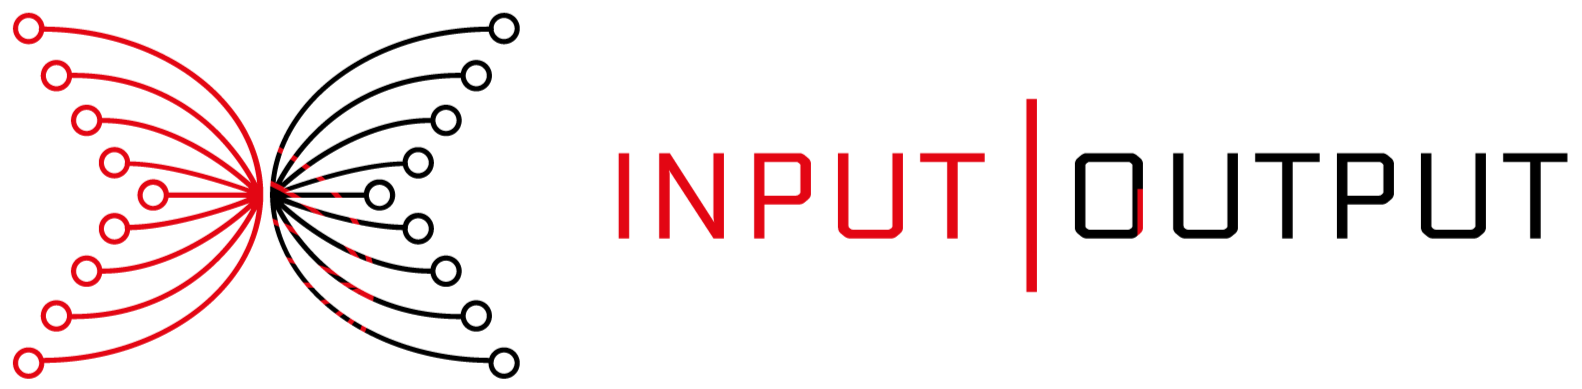
\includegraphics[scale=.375]{iohk}\hspace{.1cm}
}

\begin{document}
\begin{center}
\maketitle
\end{center}

\section{Introduction}

\begin{frame}{Motivation}
\begin{itemize}
\item A lot of blockchain applications recently
\item Sophisticated transactional schemes via \alert{smart contracts}
\item Reasoning about their execution is:
  \begin{enumerate}
  \item \textit{necessary}, significant funds are involved
  \item \textit{difficult}, due to concurrency
  \end{enumerate}
\item Hence the need for automatic tools that verify no bugs exist
  \begin{itemize}
  \item This has to be done \alert{statically}!
  \end{itemize}
\end{itemize}
\end{frame}

\begin{frame}{Background}

\begin{alertblock}{Bitcoin}
\begin{itemize}
\item Based on \textit{unspent transaction outputs} (UTxO)
\item Smart contracts in the simple language \textsc{script}
\end{itemize}
\end{alertblock}

\begin{alertblock}{Ethereum}
\begin{itemize}
\item Based on the notion of accounts
\item Smart contracts in (almost) Turing-complete Solidity/EVM
\end{itemize}
\end{alertblock}

\begin{alertblock}{Cardano (IOHK)}
\begin{itemize}
\item UTxO-based, with several extensions
\item Due to the extensions, smart contracts become more expressive
\end{itemize}
\end{alertblock}

\end{frame}

\begin{frame}{Methodology}
\begin{itemize}
\item Keep things on an abstract level
  \begin{itemize}
  \item Setup long-term foundations
  \end{itemize}
\item Fully mechanized approach, utilizing Agda's rich type system
\item Fits well with IOHK's research-oriented approach
\end{itemize}

\begin{tikzpicture}
  [basic box/.style = {
     draw,
     shape = rectangle,
     align = center,
     minimum width=2cm,
     minimum height=1.2cm,
     rounded corners},
   to/.style = {
     ->,
     >=stealth',
     semithick
  },
  every matrix/.style={column sep=.8cm, ampersand replacement=\&},
  font=\small
  ]
  \matrix{
     \node[basic box] (a) {pure\\ research};
  \& \node[basic box] (b) {mechanized\\ models};
  \& \node[basic box] (c) {reference\\ implementations};
  \& \node[basic box] (d) {production\\ code}; \\
  };

  \path
  (a) edge[to, mLightBrown] (b)
  (b) edge[to] (c)
  (c) edge[to] (d)
  ;
\end{tikzpicture}
\end{frame}
\section{Extended UTxO}
\subsection{Transactions/Ledgers}
\begin{frame}{Basic Types}
\begin{agda}\begin{hscode}\SaveRestoreHook
\column{B}{@{}>{\hspre}l<{\hspost}@{}}%
\column{3}{@{}>{\hspre}l<{\hspost}@{}}%
\column{10}{@{}>{\hspre}l<{\hspost}@{}}%
\column{21}{@{}>{\hspre}l<{\hspost}@{}}%
\column{E}{@{}>{\hspre}l<{\hspost}@{}}%
\>[B]{}\HSKeyword{module}\;\HSCon{\HSCon{UTxO}.Types}\;\HSSpecial{(}\HSCon{Value}\mathbin{:}\HSCon{Set}\HSSpecial{)}\;\HSSpecial{(}\HSCon{Hash}\mathbin{:}\HSCon{Set}\HSSpecial{)}\;\HSKeyword{where}{}\<[E]%
\\[\blanklineskip]%
\>[B]{}\HSKeyword{record}\;\HSCon{State}\mathbin{:}\HSCon{Set}\;\HSKeyword{where}{}\<[E]%
\\
\>[B]{}\hsindent{3}{}\<[3]%
\>[3]{}\HSKeyword{field}\;{}\<[10]%
\>[10]{}\HSVar{height}\mathbin{:}\HSSym{\mathbb{N}}{}\<[E]%
\\
\>[10]{}\HSSym{\vdots}{}\<[E]%
\\[\blanklineskip]%
\>[B]{}\HSKeyword{record}\;\HSCon{HashFunction}\;\HSSpecial{(}\HSCon{A}\mathbin{:}\HSCon{Set}\HSSpecial{)}\mathbin{:}\HSCon{Set}\;\HSKeyword{where}{}\<[E]%
\\
\>[B]{}\hsindent{3}{}\<[3]%
\>[3]{}\HSKeyword{field}\;{}\<[10]%
\>[10]{}\HSSym{\anonymous}\HSSym{\hspace{1pt}\#}{}\<[21]%
\>[21]{}\mathbin{:}\HSCon{A}\HSSym{\mathbin{\to}}\HSCon{Hash}{}\<[E]%
\\
\>[10]{}\HSVar{injective}{}\<[21]%
\>[21]{}\mathbin{:}\HSSym{\forall\ }\HSSpecial{\{\mskip1.5mu }\HSVar{x}\;\HSVar{y}\HSSpecial{\mskip1.5mu\}}\HSSym{\mathbin{\to}}\HSVar{x}\HSSym{\hspace{1pt}\#}\HSSym{\mathrel{\equiv}}\HSVar{y}\HSSym{\hspace{1pt}\#}\HSSym{\mathbin{\to}}\HSVar{x}\HSSym{\mathrel{\equiv}}\HSVar{y}{}\<[E]%
\\[\blanklineskip]%
\>[B]{}\HSKeyword{postulate}\;{}\<[E]%
\\
\>[B]{}\hsindent{3}{}\<[3]%
\>[3]{}\HSSym{\anonymous}\HSSym{\hspace{1pt}\#}\mathbin{:}\HSSym{\forall\ }\HSSpecial{\{\mskip1.5mu }\HSCon{A}\mathbin{:}\HSCon{Set}\HSSpecial{\mskip1.5mu\}}\HSSym{\mathbin{\to}}\HSCon{HashFunction}\;\HSCon{A}{}\<[E]%
\ColumnHook
\end{hscode}\resethooks
\end{agda}
\end{frame}

\begin{frame}{Inputs and Output References}
\begin{agda}\begin{hscode}\SaveRestoreHook
\column{B}{@{}>{\hspre}l<{\hspost}@{}}%
\column{3}{@{}>{\hspre}l<{\hspost}@{}}%
\column{10}{@{}>{\hspre}l<{\hspost}@{}}%
\column{13}{@{}>{\hspre}l<{\hspost}@{}}%
\column{17}{@{}>{\hspre}l<{\hspost}@{}}%
\column{21}{@{}>{\hspre}l<{\hspost}@{}}%
\column{E}{@{}>{\hspre}l<{\hspost}@{}}%
\>[B]{}\HSKeyword{record}\;\HSCon{TxOutputRef}\mathbin{:}\HSCon{Set}\;\HSKeyword{where}{}\<[E]%
\\
\>[B]{}\hsindent{3}{}\<[3]%
\>[3]{}\HSKeyword{constructor}\;\HSSym{\anonymous}\;\HSCon{@}\;\HSSym{\anonymous}{}\<[E]%
\\
\>[B]{}\hsindent{3}{}\<[3]%
\>[3]{}\HSKeyword{field}\;{}\<[10]%
\>[10]{}\HSVar{id}{}\<[17]%
\>[17]{}\mathbin{:}\HSCon{Hash}{}\<[E]%
\\
\>[10]{}\HSVar{index}{}\<[17]%
\>[17]{}\mathbin{:}\HSSym{\mathbb{N}}{}\<[E]%
\\[\blanklineskip]%
\>[B]{}\HSKeyword{record}\;\HSCon{TxInput}\mathbin{:}\HSCon{Set}\;\HSKeyword{where}{}\<[E]%
\\
\>[B]{}\hsindent{3}{}\<[3]%
\>[3]{}\HSKeyword{field}\;{}\<[10]%
\>[10]{}\HSVar{outputRef}{}\<[21]%
\>[21]{}\mathbin{:}\HSCon{TxOutputRef}{}\<[E]%
\\[\blanklineskip]%
\>[10]{}\HSCon{R}\;{}\<[13]%
\>[13]{}\HSCon{D}{}\<[21]%
\>[21]{}\mathbin{:}\HSSym{\mathbb{U}}{}\<[E]%
\\
\>[10]{}\HSVar{redeemer}{}\<[21]%
\>[21]{}\mathbin{:}\HSCon{State}\HSSym{\mathbin{\to}}\HSVar{el}\;\HSCon{R}{}\<[E]%
\\
\>[10]{}\HSVar{validator}{}\<[21]%
\>[21]{}\mathbin{:}\HSCon{State}\HSSym{\mathbin{\to}}\HSCon{Value}\HSSym{\mathbin{\to}}\HSCon{PendingTx}\HSSym{\mathbin{\to}}\HSVar{el}\;\HSCon{R}\HSSym{\mathbin{\to}}\HSVar{el}\;\HSCon{D}\HSSym{\mathbin{\to}}\HSCon{Bool}{}\<[E]%
\ColumnHook
\end{hscode}\resethooks
\end{agda}

\begin{itemize}
\item \ensuremath{\HSSym{\mathbb{U}}} is a simple type universe for first-order data.
\end{itemize}

\end{frame}

\begin{frame}{Transactions}
\begin{agda}\begin{hscode}\SaveRestoreHook
\column{B}{@{}>{\hspre}l<{\hspost}@{}}%
\column{3}{@{}>{\hspre}l<{\hspost}@{}}%
\column{10}{@{}>{\hspre}l<{\hspost}@{}}%
\column{14}{@{}>{\hspre}l<{\hspost}@{}}%
\column{19}{@{}>{\hspre}l<{\hspost}@{}}%
\column{22}{@{}>{\hspre}l<{\hspost}@{}}%
\column{E}{@{}>{\hspre}l<{\hspost}@{}}%
\>[B]{}\HSKeyword{module}\;\HSCon{UTxO}\;{}\<[14]%
\>[14]{}\HSSpecial{(}\HSCon{Address}\mathbin{:}\HSCon{Set}\HSSpecial{)}\;\HSSpecial{(}\HSSym{\anonymous}\HSSym{\hspace{1pt}\#}\;\HSSym{\textsub{a}}\mathbin{:}\HSCon{HashFunction}\;\HSCon{Address}\HSSpecial{)}\;{}\<[E]%
\\
\>[14]{}\HSSpecial{(}\HSSym{\anonymous}\HSSym{\mathbin{\overset{\text{\tiny ?}}{=}}}\HSSym{\textsub{a}}\;\HSSym{\anonymous}\mathbin{:}\HSCon{Decidable}\;\HSSpecial{\{\mskip1.5mu }\HSCon{A}\HSSym{\mathbin{=}}\HSCon{Address}\HSSpecial{\mskip1.5mu\}}\;\HSSym{\anonymous}\HSSym{\mathrel{\equiv}}\HSSym{\anonymous}\HSSpecial{)}\;\HSKeyword{where}{}\<[E]%
\\[\blanklineskip]%
\>[B]{}\HSKeyword{record}\;\HSCon{TxOutput}\mathbin{:}\HSCon{Set}\;\HSKeyword{where}{}\<[E]%
\\
\>[B]{}\hsindent{3}{}\<[3]%
\>[3]{}\HSKeyword{field}\;{}\<[10]%
\>[10]{}\HSVar{value}{}\<[22]%
\>[22]{}\mathbin{:}\HSCon{Value}{}\<[E]%
\\
\>[10]{}\HSVar{address}{}\<[22]%
\>[22]{}\mathbin{:}\HSCon{Address}{}\<[E]%
\\[\blanklineskip]%
\>[10]{}\HSCon{Data}{}\<[22]%
\>[22]{}\mathbin{:}\HSSym{\mathbb{U}}{}\<[E]%
\\
\>[10]{}\HSVar{dataScript}{}\<[22]%
\>[22]{}\mathbin{:}\HSCon{State}\HSSym{\mathbin{\to}}\HSVar{el}\;\HSCon{Data}{}\<[E]%
\\[\blanklineskip]%
\>[B]{}\HSKeyword{record}\;\HSCon{Tx}\mathbin{:}\HSCon{Set}\;\HSKeyword{where}{}\<[E]%
\\
\>[B]{}\hsindent{3}{}\<[3]%
\>[3]{}\HSKeyword{field}\;{}\<[10]%
\>[10]{}\HSVar{inputs}{}\<[19]%
\>[19]{}\mathbin{:}\HSCon{List}\;\HSCon{TxInput}{}\<[E]%
\\
\>[10]{}\HSVar{outputs}{}\<[19]%
\>[19]{}\mathbin{:}\HSCon{List}\;\HSCon{TxOutput}{}\<[E]%
\\
\>[10]{}\HSVar{forge}{}\<[19]%
\>[19]{}\mathbin{:}\HSCon{Value}{}\<[E]%
\\
\>[10]{}\HSVar{fee}{}\<[19]%
\>[19]{}\mathbin{:}\HSCon{Value}{}\<[E]%
\\[\blanklineskip]%
\>[B]{}\HSCon{Ledger}\mathbin{:}\HSCon{Set}{}\<[E]%
\\
\>[B]{}\HSCon{Ledger}\HSSym{\mathbin{=}}\HSCon{List}\;\HSCon{Tx}{}\<[E]%
\ColumnHook
\end{hscode}\resethooks
\end{agda}
\end{frame}

\begin{frame}{Validation}
\begin{agda}\begin{hscode}\SaveRestoreHook
\column{B}{@{}>{\hspre}l<{\hspost}@{}}%
\column{3}{@{}>{\hspre}l<{\hspost}@{}}%
\column{11}{@{}>{\hspre}c<{\hspost}@{}}%
\column{11E}{@{}l@{}}%
\column{14}{@{}>{\hspre}l<{\hspost}@{}}%
\column{E}{@{}>{\hspre}l<{\hspost}@{}}%
\>[B]{}\HSVar{validate}{}\<[11]%
\>[11]{}\mathbin{:}{}\<[11E]%
\>[14]{}\HSCon{PendingTx}{}\<[E]%
\\
\>[11]{}\HSSym{\mathbin{\to}}{}\<[11E]%
\>[14]{}\HSSpecial{(}\HSVar{i}\mathbin{:}\HSCon{TxInput}\HSSpecial{)}{}\<[E]%
\\
\>[11]{}\HSSym{\mathbin{\to}}{}\<[11E]%
\>[14]{}\HSSpecial{(}\HSVar{o}\mathbin{:}\HSCon{TxOutput}\HSSpecial{)}{}\<[E]%
\\
\>[11]{}\HSSym{\mathbin{\to}}{}\<[11E]%
\>[14]{}\HSCon{D}\;\HSVar{i}\HSSym{\mathrel{\equiv}}\HSCon{Data}\;\HSVar{o}{}\<[E]%
\\
\>[11]{}\HSSym{\mathbin{\to}}{}\<[11E]%
\>[14]{}\HSCon{State}{}\<[E]%
\\
\>[11]{}\HSSym{\mathbin{\to}}{}\<[11E]%
\>[14]{}\HSCon{Bool}{}\<[E]%
\\
\>[B]{}\HSVar{validate}\;\HSVar{ptx}\;\HSVar{i}\;\HSVar{o}\;\HSCon{refl}\;\HSVar{st}\HSSym{\mathbin{=}}{}\<[E]%
\\
\>[B]{}\hsindent{3}{}\<[3]%
\>[3]{}\HSVar{validator}\;\HSVar{i}\;\HSVar{st}\;\HSSpecial{(}\HSVar{value}\;\HSVar{o}\HSSpecial{)}\;\HSVar{ptx}\;\HSSpecial{(}\HSVar{redeemer}\;\HSVar{i}\;\HSVar{st}\HSSpecial{)}\;\HSSpecial{(}\HSVar{dataScript}\;\HSVar{o}\;\HSVar{st}\HSSpecial{)}{}\<[E]%
\ColumnHook
\end{hscode}\resethooks
\end{agda}
\end{frame}

\begin{frame}{Unspent Outputs}
\begin{agda}\begin{hscode}\SaveRestoreHook
\column{B}{@{}>{\hspre}l<{\hspost}@{}}%
\column{3}{@{}>{\hspre}l<{\hspost}@{}}%
\column{5}{@{}>{\hspre}l<{\hspost}@{}}%
\column{26}{@{}>{\hspre}l<{\hspost}@{}}%
\column{28}{@{}>{\hspre}l<{\hspost}@{}}%
\column{E}{@{}>{\hspre}l<{\hspost}@{}}%
\>[B]{}\HSVar{unspentOutputs}\mathbin{:}\HSCon{Ledger}\HSSym{\mathbin{\to}}\HSCon{Set}\HSSym{\langle\ }\HSCon{TxOutputRef}\HSSym{\ \rangle}{}\<[E]%
\\
\>[B]{}\HSVar{unspentOutputs}\;\HSSpecial{[\mskip1.5mu }\HSSpecial{\mskip1.5mu]}{}\<[28]%
\>[28]{}\HSSym{\mathbin{=}}\HSSym{\varnothing}{}\<[E]%
\\
\>[B]{}\HSVar{unspentOutputs}\;\HSSpecial{(}\HSVar{tx}\HSCon{::}\HSVar{txs}\HSSpecial{)}{}\<[28]%
\>[28]{}\HSSym{\mathbin{=}}\HSSpecial{(}\HSVar{unspentOutputs}\;\HSVar{txs}\HSSym{\mathbin{\setminus}}\HSVar{spentOutputsTx}\;\HSVar{tx}\HSSpecial{)}{}\<[E]%
\\
\>[28]{}\HSSym{\mathbin{\cup}}\HSVar{unspentOutputsTx}\;\HSVar{tx}{}\<[E]%
\\
\>[B]{}\hsindent{3}{}\<[3]%
\>[3]{}\HSKeyword{where}{}\<[E]%
\\
\>[3]{}\hsindent{2}{}\<[5]%
\>[5]{}\HSVar{spentOutputsTx}\HSSpecial{\HSSym{\mathbin{,}}}\HSVar{unspentOutputsTx}\mathbin{:}\HSCon{Tx}\HSSym{\mathbin{\to}}\HSCon{Set}\HSSym{\langle\ }\HSCon{TxOutputRef}\HSSym{\ \rangle}{}\<[E]%
\\
\>[3]{}\hsindent{2}{}\<[5]%
\>[5]{}\HSVar{spentOutputsTx}{}\<[26]%
\>[26]{}\HSSym{\mathbin{=}}\HSSpecial{(}\HSVar{outputRef}\HSSym{\mathrel{\langle\$\rangle}}\HSSym{\!\_}\HSSpecial{)}\HSSym{\mathbin{\circ}}\HSVar{inputs}{}\<[E]%
\\
\>[3]{}\hsindent{2}{}\<[5]%
\>[5]{}\HSVar{unspentOutputsTx}\;\HSVar{tx}{}\<[26]%
\>[26]{}\HSSym{\mathbin{=}}\HSSpecial{(}\HSVar{tx}\HSSym{\hspace{1pt}\#}\;\HSCon{@}\;\HSSym{\!\_}\HSSpecial{)}\HSSym{\mathrel{\langle\$\rangle}}\HSVar{indices}\;\HSSpecial{(}\HSVar{outputs}\;\HSVar{tx}\HSSpecial{)}{}\<[E]%
\ColumnHook
\end{hscode}\resethooks
\end{agda}
\end{frame}

\subsection{Validity}
\begin{frame}{Validity I}
\begin{agda}\begin{hscode}\SaveRestoreHook
\column{B}{@{}>{\hspre}l<{\hspost}@{}}%
\column{3}{@{}>{\hspre}l<{\hspost}@{}}%
\column{5}{@{}>{\hspre}l<{\hspost}@{}}%
\column{7}{@{}>{\hspre}l<{\hspost}@{}}%
\column{E}{@{}>{\hspre}l<{\hspost}@{}}%
\>[B]{}\HSKeyword{record}\;\HSCon{IsValidTx}\;\HSSpecial{(}\HSVar{tx}\mathbin{:}\HSCon{Tx}\HSSpecial{)}\;\HSSpecial{(}\HSVar{l}\mathbin{:}\HSCon{Ledger}\HSSpecial{)}\mathbin{:}\HSCon{Set}\;\HSKeyword{where}{}\<[E]%
\\
\>[B]{}\HSKeyword{field}\;{}\<[E]%
\\
\>[B]{}\hsindent{3}{}\<[3]%
\>[3]{}\HSCon{validTxRefs}\mathbin{:}\HSSym{\forall\ }\HSVar{i}\HSSym{\mathbin{\to}}\HSVar{i}\HSSym{\mathrel{\in}}\HSVar{inputs}\;\HSVar{tx}\to {}\<[E]%
\\
\>[3]{}\hsindent{2}{}\<[5]%
\>[5]{}\HSCon{Any}\;\HSSpecial{(}\HSVar{λ}\;\HSVar{t}\HSSym{\mathbin{\to}}\HSVar{t}\HSSym{\hspace{1pt}\#}\HSSym{\mathrel{\equiv}}\HSVar{id}\;\HSSpecial{(}\HSVar{outputRef}\;\HSVar{i}\HSSpecial{)}\HSSpecial{)}\;\HSVar{l}{}\<[E]%
\\[\blanklineskip]%
\>[B]{}\hsindent{3}{}\<[3]%
\>[3]{}\HSCon{validOutputIndices}\mathbin{:}\HSSym{\forall\ }\HSVar{i}\HSSym{\mathbin{\to}}\HSSpecial{(}\HSVar{i\!\in}\mathbin{:}\HSVar{i}\HSSym{\mathrel{\in}}\HSVar{inputs}\;\HSVar{tx}\HSSpecial{)}\to {}\<[E]%
\\
\>[3]{}\hsindent{2}{}\<[5]%
\>[5]{}\HSVar{index}\;\HSSpecial{(}\HSVar{outputRef}\;\HSVar{i}\HSSpecial{)}\HSSym{<}{}\<[E]%
\\
\>[5]{}\hsindent{2}{}\<[7]%
\>[7]{}\HSVar{length}\;\HSSpecial{(}\HSVar{outputs}\;\HSSpecial{(}\HSVar{lookupTx}\;\HSVar{l}\;\HSSpecial{(}\HSVar{outputRef}\;\HSVar{i}\HSSpecial{)}\;\HSSpecial{(}\HSCon{validTxRefs}\;\HSVar{i}\;\HSVar{i\!\in}\HSSpecial{)}\HSSpecial{)}\HSSpecial{)}{}\<[E]%
\\[\blanklineskip]%
\>[B]{}\hsindent{3}{}\<[3]%
\>[3]{}\HSCon{validOutputRefs}\mathbin{:}\HSSym{\forall\ }\HSVar{i}\HSSym{\mathbin{\to}}\HSVar{i}\HSSym{\mathrel{\in}}\HSVar{inputs}\;\HSVar{tx}\to {}\<[E]%
\\
\>[3]{}\hsindent{2}{}\<[5]%
\>[5]{}\HSVar{outputRef}\;\HSVar{i}\HSSym{\mathrel{\in}}\HSVar{unspentOutputs}\;\HSVar{l}{}\<[E]%
\\[\blanklineskip]%
\>[B]{}\hsindent{3}{}\<[3]%
\>[3]{}\HSCon{validDataScriptTypes}\mathbin{:}\HSSym{\forall\ }\HSVar{i}\HSSym{\mathbin{\to}}\HSSpecial{(}\HSVar{i\!\in}\mathbin{:}\HSVar{i}\HSSym{\mathrel{\in}}\HSVar{inputs}\;\HSVar{tx}\HSSpecial{)}\to {}\<[E]%
\\
\>[3]{}\hsindent{2}{}\<[5]%
\>[5]{}\HSCon{D}\;\HSVar{i}\HSSym{\mathrel{\equiv}}\HSCon{D}\;\HSSpecial{(}\HSVar{lookupOutput}\;\HSVar{l}\;\HSSpecial{(}\HSVar{outputRef}\;\HSVar{i}\HSSpecial{)}\;\HSSym{\dots}\HSSpecial{)}{}\<[E]%
\ColumnHook
\end{hscode}\resethooks
\end{agda}
\end{frame}

\begin{frame}{Validity II}
\begin{agda}\begin{hscode}\SaveRestoreHook
\column{B}{@{}>{\hspre}l<{\hspost}@{}}%
\column{3}{@{}>{\hspre}l<{\hspost}@{}}%
\column{5}{@{}>{\hspre}c<{\hspost}@{}}%
\column{5E}{@{}l@{}}%
\column{8}{@{}>{\hspre}l<{\hspost}@{}}%
\column{E}{@{}>{\hspre}l<{\hspost}@{}}%
\>[B]{}\HSCon{preservesValues}\mathbin{:}{}\<[E]%
\\
\>[B]{}\hsindent{3}{}\<[3]%
\>[3]{}\HSVar{forge}\;\HSVar{tx}\HSSym{+}\HSVar{sum}\;\HSSpecial{(}\HSVar{lookupValue}\;\HSVar{l}\;\HSSym{\dots}\HSSym{\mathrel{\langle\$\rangle}}\HSVar{inputs}\;\HSVar{tx}\HSSpecial{)}{}\<[E]%
\\
\>[3]{}\hsindent{2}{}\<[5]%
\>[5]{}\HSSym{\mathrel{\equiv}}{}\<[5E]%
\\
\>[B]{}\hsindent{3}{}\<[3]%
\>[3]{}\HSVar{fee}\;\HSVar{tx}\HSSym{+}\HSVar{sum}\;\HSSpecial{(}\HSVar{value}\HSSym{\mathrel{\langle\$\rangle}}\HSVar{outputs}\;\HSVar{tx}\HSSpecial{)}{}\<[E]%
\\[\blanklineskip]%
\>[B]{}\HSCon{noDoubleSpending}\mathbin{:}{}\<[E]%
\\
\>[B]{}\hsindent{3}{}\<[3]%
\>[3]{}\HSVar{noDuplicates}\;\HSSpecial{(}\HSVar{outputRef}\HSSym{\mathrel{\langle\$\rangle}}\HSVar{inputs}\;\HSVar{tx}\HSSpecial{)}{}\<[E]%
\\[\blanklineskip]%
\>[B]{}\HSCon{allInputsValidate}\mathbin{:}\HSSym{\forall\ }\HSVar{i}\HSSym{\mathbin{\to}}\HSSpecial{(}\HSVar{i\!\in}\mathbin{:}\HSVar{i}\HSSym{\mathrel{\in}}\HSVar{inputs}\;\HSVar{tx}\HSSpecial{)}\to {}\<[E]%
\\
\>[B]{}\hsindent{3}{}\<[3]%
\>[3]{}\HSKeyword{let}\;{}\<[8]%
\>[8]{}\HSVar{out}\HSSym{\mathbin{=}}\HSVar{lookupOutput}\;\HSVar{l}\;\HSSpecial{(}\HSVar{outputRef}\;\HSVar{i}\HSSpecial{)}\;\HSSym{\dots}{}\<[E]%
\\
\>[8]{}\HSVar{ptx}\HSSym{\mathbin{=}}\HSVar{mkPendingTx}\;\HSVar{l}\;\HSVar{tx}\;\HSCon{validTxRefs}\;\HSCon{validOutputIndices}{}\<[E]%
\\
\>[B]{}\hsindent{3}{}\<[3]%
\>[3]{}\HSKeyword{in}\;{}\<[8]%
\>[8]{}\HSCon{T}\;\HSSpecial{(}\HSVar{validate}\;\HSVar{ptx}\;\HSVar{i}\;\HSVar{out}\;\HSSpecial{(}\HSCon{validDataScriptTypes}\;\HSVar{i}\;\HSVar{i\!\in}\HSSpecial{)}\;\HSSpecial{(}\HSVar{getState}\;\HSVar{l}\HSSpecial{)}\HSSpecial{)}{}\<[E]%
\\[\blanklineskip]%
\>[B]{}\HSCon{validateValidHashes}\mathbin{:}\HSSym{\forall\ }\HSVar{i}\HSSym{\mathbin{\to}}\HSSpecial{(}\HSVar{i\!\in}\mathbin{:}\HSVar{i}\HSSym{\mathrel{\in}}\HSVar{inputs}\;\HSVar{tx}\HSSpecial{)}\to {}\<[E]%
\\
\>[B]{}\hsindent{3}{}\<[3]%
\>[3]{}\HSKeyword{let}\;{}\<[8]%
\>[8]{}\HSVar{out}\HSSym{\mathbin{=}}\HSVar{lookupOutput}\;\HSVar{l}\;\HSSpecial{(}\HSVar{outputRef}\;\HSVar{i}\HSSpecial{)}\;\HSSym{\dots}{}\<[E]%
\\
\>[B]{}\hsindent{3}{}\<[3]%
\>[3]{}\HSKeyword{in}\;{}\<[8]%
\>[8]{}\HSSpecial{(}\HSVar{address}\;\HSVar{out}\HSSpecial{)}\HSSym{\hspace{1pt}\#}\HSSym{\mathrel{\equiv}}\HSVar{validator}\;\HSVar{i}\HSSym{\hspace{1pt}\#}{}\<[E]%
\ColumnHook
\end{hscode}\resethooks
\end{agda}
\end{frame}

\begin{frame}{Valid Ledgers}
We do not want a ledger to be any list of transactions,
but a ``snoc''-list that carries proofs of validity:
\begin{agda}\begin{hscode}\SaveRestoreHook
\column{B}{@{}>{\hspre}l<{\hspost}@{}}%
\column{3}{@{}>{\hspre}l<{\hspost}@{}}%
\column{15}{@{}>{\hspre}c<{\hspost}@{}}%
\column{15E}{@{}l@{}}%
\column{18}{@{}>{\hspre}l<{\hspost}@{}}%
\column{E}{@{}>{\hspre}l<{\hspost}@{}}%
\>[B]{}\HSKeyword{data}\;\HSCon{ValidLedger}\mathbin{:}\HSCon{Ledger}\HSSym{\mathbin{\to}}\HSCon{Set}\;\HSKeyword{where}{}\<[E]%
\\[\blanklineskip]%
\>[B]{}\hsindent{3}{}\<[3]%
\>[3]{}\HSSym{\mathlarger{\mathlarger{\mathlarger{\cdot}}}}{}\<[15]%
\>[15]{}\mathbin{:}{}\<[15E]%
\>[18]{}\HSCon{ValidLedger}\;\HSSpecial{[\mskip1.5mu }\HSSpecial{\mskip1.5mu]}{}\<[E]%
\\[\blanklineskip]%
\>[B]{}\hsindent{3}{}\<[3]%
\>[3]{}\HSSym{\anonymous}\HSSym{\mathbin{\oplus}}\HSSym{\anonymous}\HSSym{\dashv}\HSSym{\anonymous}{}\<[15]%
\>[15]{}\mathbin{:}{}\<[15E]%
\>[18]{}\HSCon{ValidLedger}\;\HSVar{l}{}\<[E]%
\\
\>[15]{}\HSSym{\mathbin{\to}}{}\<[15E]%
\>[18]{}\HSSpecial{(}\HSVar{tx}\mathbin{:}\HSCon{Tx}\HSSpecial{)}{}\<[E]%
\\
\>[15]{}\HSSym{\mathbin{\to}}{}\<[15E]%
\>[18]{}\HSCon{IsValidTx}\;\HSVar{tx}\;\HSVar{l}{}\<[E]%
\\
\>[15]{}\HSSym{\mathbin{\to}}{}\<[15E]%
\>[18]{}\HSCon{ValidLedger}\;\HSSpecial{(}\HSVar{tx}\HSCon{::}\HSVar{l}\HSSpecial{)}{}\<[E]%
\ColumnHook
\end{hscode}\resethooks
\end{agda}
\end{frame}

\begin{frame}{Decision Procedures}
\begin{agda}\begin{hscode}\SaveRestoreHook
\column{B}{@{}>{\hspre}l<{\hspost}@{}}%
\column{3}{@{}>{\hspre}l<{\hspost}@{}}%
\column{5}{@{}>{\hspre}c<{\hspost}@{}}%
\column{5E}{@{}l@{}}%
\column{9}{@{}>{\hspre}c<{\hspost}@{}}%
\column{9E}{@{}l@{}}%
\column{12}{@{}>{\hspre}l<{\hspost}@{}}%
\column{E}{@{}>{\hspre}l<{\hspost}@{}}%
\>[B]{}\HSSym{\vdots}{}\<[E]%
\\
\>[B]{}\HSCon{validOutputRefs}\HSSym{?}\mathbin{:}\HSSym{\forall\ }\HSSpecial{(}\HSVar{tx}\mathbin{:}\HSCon{Tx}\HSSpecial{)}\;\HSSpecial{(}\HSVar{l}\mathbin{:}\HSCon{Ledger}\HSSpecial{)}{}\<[E]%
\\
\>[B]{}\hsindent{3}{}\<[3]%
\>[3]{}\HSSym{\mathbin{\to}}\HSCon{Dec}\;\HSSpecial{(}\HSSym{\forall\ }\HSVar{i}\HSSym{\mathbin{\to}}\HSVar{i}\HSSym{\mathrel{\in}}\HSVar{inputs}\;\HSVar{tx}\HSSym{\mathbin{\to}}\HSVar{outputRef}\;\HSVar{i}\HSSym{\mathrel{\in}}\HSVar{unspentOutputs}\;\HSVar{l}\HSSpecial{)}{}\<[E]%
\\
\>[B]{}\HSCon{validOutputRefs}\HSSym{?}\HSVar{tx}\;\HSVar{l}\HSSym{\mathbin{=}}{}\<[E]%
\\
\>[B]{}\hsindent{3}{}\<[3]%
\>[3]{}\HSSym{\forall ?\ }\HSSpecial{(}\HSVar{inputs}\;\HSVar{tx}\HSSpecial{)}\;\HSVar{λ}\;\HSVar{i}\;\HSSym{\anonymous}\HSSym{\mathbin{\to}}\HSVar{outputRef}\;\HSVar{i}\HSSym{\mathrel{\in ?}}\HSVar{unspentOutputs}\;\HSVar{l}{}\<[E]%
\\
\>[B]{}\hsindent{3}{}\<[3]%
\>[3]{}\HSSym{\vdots}{}\<[E]%
\\
\>[B]{}\hsindent{3}{}\<[3]%
\>[3]{}\HSKeyword{where}{}\<[E]%
\\
\>[3]{}\hsindent{2}{}\<[5]%
\>[5]{}\HSSym{\forall ?\ }{}\<[5E]%
\>[9]{}\mathbin{:}{}\<[9E]%
\>[12]{}\HSSpecial{(}\HSVar{xs}\mathbin{:}\HSCon{List}\;\HSCon{A}\HSSpecial{)}{}\<[E]%
\\
\>[9]{}\HSSym{\mathbin{\to}}{}\<[9E]%
\>[12]{}\HSSpecial{\{\mskip1.5mu }\HSCon{P}\mathbin{:}\HSSpecial{(}\HSVar{x}\mathbin{:}\HSCon{A}\HSSpecial{)}\;\HSSpecial{(}\HSVar{x\!\in}\mathbin{:}\HSVar{x}\HSSym{\mathrel{\in}}\HSVar{xs}\HSSpecial{)}\HSSym{\mathbin{\to}}\HSCon{Set}\HSSpecial{\mskip1.5mu\}}{}\<[E]%
\\
\>[9]{}\HSSym{\mathbin{\to}}{}\<[9E]%
\>[12]{}\HSSpecial{(}\HSSym{\forall\ }\HSVar{x}\HSSym{\mathbin{\to}}\HSSpecial{(}\HSVar{x\!\in}\mathbin{:}\HSVar{x}\HSSym{\mathrel{\in}}\HSVar{xs}\HSSpecial{)}\HSSym{\mathbin{\to}}\HSCon{Dec}\;\HSSpecial{(}\HSCon{P}\;\HSVar{x}\;\HSVar{x\!\in}\HSSpecial{)}\HSSpecial{)}{}\<[E]%
\\
\>[9]{}\HSSym{\mathbin{\to}}{}\<[9E]%
\>[12]{}\HSCon{Dec}\;\HSSpecial{(}\HSSym{\forall\ }\HSVar{x}\;\HSVar{x\!\in}\HSSym{\mathbin{\to}}\HSCon{P}\;\HSVar{x}\;\HSVar{x\!\in}\HSSpecial{)}{}\<[E]%
\ColumnHook
\end{hscode}\resethooks
\end{agda}
\end{frame}


\subsection{Extensions}

\begin{frame}{Extension: Multi-currency}
\begin{enumerate}
\item Generalize values from integers to maps: \ensuremath{\HSCon{Value}\HSSym{\mathbin{=}}\HSCon{List}\;\HSSpecial{(}\HSCon{Hash}\HSSym{\mathrel{\times}}\HSSym{\mathbb{N}}\HSSpecial{)}}
\item Implement additive group operators (on top of AVL trees):
\begin{agda}\begin{hscode}\SaveRestoreHook
\column{B}{@{}>{\hspre}l<{\hspost}@{}}%
\column{3}{@{}>{\hspre}l<{\hspost}@{}}%
\column{5}{@{}>{\hspre}l<{\hspost}@{}}%
\column{E}{@{}>{\hspre}l<{\hspost}@{}}%
\>[B]{}\HSKeyword{open}\;\HSKeyword{import}\;\HSCon{\HSCon{Data}.AVL}\;\HSSym{\mathbb{N}}\HSSym{\text{\textit{-}}}\HSVar{strictTotalOrder}{}\<[E]%
\\[\blanklineskip]%
\>[B]{}\HSSym{\anonymous}\HSSym{+}\HSSym{\textsup{c}}\;\HSSym{\anonymous}\mathbin{:}\HSCon{Value}\HSSym{\mathbin{\to}}\HSCon{Value}\HSSym{\mathbin{\to}}\HSCon{Value}{}\<[E]%
\\
\>[B]{}\HSVar{c}\HSSym{+}\HSSym{\textsup{c}}\;\HSVar{c}\hspace{2pt}^{\mathsmaller{\prime}}\HSSym{\mathbin{=}}\HSVar{toList}\;\HSSpecial{(}\HSVar{foldl}\;\HSVar{go}\;\HSSpecial{(}\HSVar{fromList}\;\HSVar{c}\HSSpecial{)}\;\HSVar{c}\hspace{2pt}^{\mathsmaller{\prime}}\HSSpecial{)}{}\<[E]%
\\
\>[B]{}\hsindent{3}{}\<[3]%
\>[3]{}\HSKeyword{where}{}\<[E]%
\\
\>[3]{}\hsindent{2}{}\<[5]%
\>[5]{}\HSVar{go}\mathbin{:}\HSCon{Tree}\;\HSCon{Hash}\;\HSSym{\mathbb{N}}\HSSym{\mathbin{\to}}\HSSpecial{(}\HSCon{Hash}\HSSym{\mathrel{\times}}\HSSym{\mathbb{N}}\HSSpecial{)}\HSSym{\mathbin{\to}}\HSCon{Tree}\;\HSCon{Hash}\;\HSSym{\mathbb{N}}{}\<[E]%
\\
\>[3]{}\hsindent{2}{}\<[5]%
\>[5]{}\HSVar{go}\;\HSVar{m}\;\HSSpecial{(}\HSVar{k}\HSSpecial{\HSSym{\mathbin{,}}}\HSVar{v}\HSSpecial{)}\HSSym{\mathbin{=}}\HSVar{insertWith}\;\HSVar{k}\;\HSSpecial{(}\HSSpecial{(}\HSSym{\_\!}\HSSym{+}\HSVar{v}\HSSpecial{)}\HSSym{\mathbin{\circ}}\HSVar{fromMaybe}\;\HSNumeral{0}\HSSpecial{)}\;\HSVar{m}{}\<[E]%
\\[\blanklineskip]%
\>[B]{}\HSVar{sum}\;\HSSym{\textsup{c}}\mathbin{:}\HSCon{Values}\HSSym{\mathbin{\to}}\HSCon{Value}{}\<[E]%
\\
\>[B]{}\HSVar{sum}\;\HSSym{\textsup{c}}\HSSym{\mathbin{=}}\HSVar{foldl}\;\HSSym{\_\!}\HSSym{+}\HSSym{\textsup{c}}\;\HSSym{\!\_}\;\HSSpecial{[\mskip1.5mu }\HSSpecial{\mskip1.5mu]}{}\<[E]%
\ColumnHook
\end{hscode}\resethooks
\end{agda}
\end{enumerate}
\end{frame}

\begin{frame}{Multi-currency: Forging condition}
We now need to enforce monetary policies on forging transactions:
\begin{agda}\begin{hscode}\SaveRestoreHook
\column{B}{@{}>{\hspre}l<{\hspost}@{}}%
\column{3}{@{}>{\hspre}l<{\hspost}@{}}%
\column{5}{@{}>{\hspre}l<{\hspost}@{}}%
\column{7}{@{}>{\hspre}l<{\hspost}@{}}%
\column{9}{@{}>{\hspre}l<{\hspost}@{}}%
\column{E}{@{}>{\hspre}l<{\hspost}@{}}%
\>[B]{}\HSKeyword{record}\;\HSCon{IsValidTx}\;\HSSpecial{(}\HSVar{tx}\mathbin{:}\HSCon{Tx}\HSSpecial{)}\;\HSSpecial{(}\HSVar{l}\mathbin{:}\HSCon{Ledger}\HSSpecial{)}\mathbin{:}\HSCon{Set}\;\HSKeyword{where}{}\<[E]%
\\
\>[B]{}\hsindent{3}{}\<[3]%
\>[3]{}\HSSym{\vdots}{}\<[E]%
\\
\>[B]{}\hsindent{3}{}\<[3]%
\>[3]{}\HSCon{forging}\mathbin{:}{}\<[E]%
\\
\>[3]{}\hsindent{2}{}\<[5]%
\>[5]{}\HSSym{\forall\ }\HSVar{c}\HSSym{\mathbin{\to}}\HSVar{c}\HSSym{\mathrel{\in}}\HSVar{keys}\;\HSSpecial{(}\HSVar{forge}\;\HSVar{tx}\HSSpecial{)}\HSSym{\mathbin{\to}}{}\<[E]%
\\
\>[5]{}\hsindent{2}{}\<[7]%
\>[7]{}\HSSym{\exists}\HSSpecial{[\mskip1.5mu }\HSVar{i}\HSSpecial{\mskip1.5mu]}\;\HSSym{\exists}\HSVar{λ}\;\HSSpecial{(}\HSVar{i\!\in}\mathbin{:}\HSVar{i}\HSSym{\mathrel{\in}}\HSVar{inputs}\;\HSVar{tx}\HSSpecial{)}\HSSym{\mathbin{\to}}{}\<[E]%
\\
\>[7]{}\hsindent{2}{}\<[9]%
\>[9]{}\HSKeyword{let}\;\HSVar{out}\HSSym{\mathbin{=}}\HSVar{lookupOutput}\;\HSVar{l}\;\HSSpecial{(}\HSVar{outputRef}\;\HSVar{i}\HSSpecial{)}\;\HSSym{\dots}{}\<[E]%
\\
\>[7]{}\hsindent{2}{}\<[9]%
\>[9]{}\HSKeyword{in}\;\HSSpecial{(}\HSVar{address}\;\HSVar{out}\HSSpecial{)}\HSSym{\hspace{1pt}\#}\HSSym{\mathrel{\equiv}}\HSVar{c}{}\<[E]%
\ColumnHook
\end{hscode}\resethooks
\end{agda}
\end{frame}

\subsection{Example}
\newcommand\forge[1]{forge: \bitcoin ~#1}
\newcommand\fee[1]{fee:\hspace{7pt} \bitcoin ~#1}
\begin{frame}{Example: Transaction Graph}
\begin{figure}\begin{tikzpicture}
  [transform canvas={scale=0.8},
   basic box/.style = {
     draw,
     shape = rectangle,
     align = left,
     minimum width=2cm,
     minimum height=1.2cm,
     rounded corners},
   upedge/.style = {
     },
   downedge/.style = {
     },
   to/.style = {
     ->,
     >=stealth',
     semithick
  },
  every matrix/.style={column sep=1.3cm, row sep=1cm, ampersand replacement=\&},
  font=\footnotesize
  ]
  \matrix{
    \node[basic box, label = \ensuremath{\HSVar{t}\;\textsub{1}}] (t)
      {\forge{1000}\\ \fee{0}};
    \& \node[basic box, label = \ensuremath{\HSVar{t}\;\textsub{2}}] (tt)
      {\forge{0}\\ \fee{0}};
    \& \node[basic box, label = \ensuremath{\HSVar{t}\;\textsub{5}}] (tfive)
      {\forge{0}\\ \fee{7}};
    \& \node[basic box, label = \ensuremath{\HSVar{t}\;\textsub{6}}] (tsix)
      {\forge{0}\\ \fee{1}};
    \& \node (end) {}; \\

    \node {};
    \& \node[basic box, label = \ensuremath{\HSVar{t}\;\textsub{3}}] (ttt)
      {\forge{0}\\ \fee{1}};
    \& \node {};
    \& \node {}; \\

    \node {};
    \& \node[basic box, label = \ensuremath{\HSVar{t}\;\textsub{4}}] (tfour)
      {\forge{10}\\ \fee{2}};
    \& \node {};
    \& \node {}; \\
  };

  \path
  (t) edge[to]
    node[above]{\bitcoin ~1000}
    node[below]{@\ensuremath{\HSSym{\mathbb{A}}}}
  (tt)
  (tt) edge[to, bend right = 30]
    node[left]{\bitcoin ~200}
    node[right]{@\ensuremath{\HSSym{\mathbb{A}}}}
  (ttt)
  (tt) edge[to]
    node[above]{\bitcoin ~800}
    node[below]{@\ensuremath{\HSSym{\mathbb{B}}}}
  (tfive)
  (ttt) edge[to, bend right = 30]
    node[left]{\bitcoin ~199}
    node[right]{@\ensuremath{\HSSym{\mathbb{C}}}}
  (tfour)
  (tfour) edge[to, bend right = 45]
    node[left]{\bitcoin ~207}
    node[right]{@\ensuremath{\HSSym{\mathbb{B}}}}
  (tfive)
  (tfive) edge[to, transform canvas={yshift=13pt}]
    node[above]{\bitcoin ~500}
    node[below]{@\ensuremath{\HSSym{\mathbb{B}}}}
  (tsix)
  (tfive) edge[to, transform canvas={yshift=-13pt}]
    node[above]{\bitcoin ~500}
    node[below]{@\ensuremath{\HSSym{\mathbb{C}}}}
  (tsix)
  (tsix) edge[to, red]
    node[above,black]{\bitcoin ~999}
    node[below,black]{@\ensuremath{\HSSym{\mathbb{C}}}}
  (end)
  ;
\end{tikzpicture}\end{figure}
\end{frame}

\begin{frame}{Example: Transaction Graph \alert{+ monetary policy}}
\begin{figure}\begin{tikzpicture}
  [transform canvas={scale=0.8},
   basic box/.style = {
     draw,
     shape = rectangle,
     align = left,
     minimum width=2cm,
     minimum height=1.2cm,
     rounded corners},
   upedge/.style = {
     },
   downedge/.style = {
     },
   to/.style = {
     ->,
     >=stealth',
     semithick
  },
  every matrix/.style={column sep=1.3cm, row sep=1cm, ampersand replacement=\&},
  font=\footnotesize
  ]
  \matrix{
    \node[basic box, label = \ensuremath{\HSVar{t}\;\textsub{1}}] (t)
      {\forge{1000}\\ \fee{0}};
    \& \node[basic box, label = \ensuremath{\HSVar{t}\;\textsub{2}}] (tt)
      {\forge{0}\\ \fee{0}};
    \& \node[basic box, label = \ensuremath{\HSVar{t}\;\textsub{5}}] (tfive)
      {\forge{0}\\ \fee{7}};
    \& \node[basic box, label = \ensuremath{\HSVar{t}\;\textsub{6}}] (tsix)
      {\forge{0}\\ \fee{1}};
    \& \node (end) {}; \\

    \node[basic box, label = \ensuremath{\HSVar{c}\;\textsub{0}}] (c)
      {\forge{0}\\ \fee{0}};
    \& \node[basic box, label = \ensuremath{\HSVar{t}\;\textsub{3}}] (ttt)
      {\forge{0}\\ \fee{1}};
    \& \node {};
    \& \node {}; \\

    \node {};
    \& \node[basic box, label = \ensuremath{\HSVar{t}\;\textsub{4}}] (tfour)
      {\forge{10}\\ \fee{2}};
    \& \node {};
    \& \node {}; \\
  };

  \path
  (t) edge[to]
    node[above]{\bitcoin ~1000}
    node[below]{@\ensuremath{\HSSym{\mathbb{A}}}}
  (tt)
  (tt) edge[to, bend right = 30]
    node[left]{\bitcoin ~200}
    node[right]{@\ensuremath{\HSSym{\mathbb{A}}}}
  (ttt)
  (tt) edge[to]
    node[above]{\bitcoin ~800}
    node[below]{@\ensuremath{\HSSym{\mathbb{B}}}}
  (tfive)
  (ttt) edge[to, bend right = 30]
    node[left]{\bitcoin ~199}
    node[right]{@\ensuremath{\HSSym{\mathbb{C}}}}
  (tfour)
  (tfour) edge[to, bend right = 45]
    node[left]{\bitcoin ~207}
    node[right]{@\ensuremath{\HSSym{\mathbb{B}}}}
  (tfive)
  (tfive) edge[to, transform canvas={yshift=13pt}]
    node[above]{\bitcoin ~500}
    node[below]{@\ensuremath{\HSSym{\mathbb{B}}}}
  (tsix)
  (tfive) edge[to, transform canvas={yshift=-13pt}]
    node[above]{\bitcoin ~500}
    node[below]{@\ensuremath{\HSSym{\mathbb{C}}}}
  (tsix)
  (tsix) edge[to, red]
    node[above,black]{\bitcoin ~999}
    node[below,black]{@\ensuremath{\HSSym{\mathbb{C}}}}
  (end)
  (c) edge[to, bend left = 30, green]
    node[left,black]{\bitcoin-policy}
    node[right,black]{@\ensuremath{\HSSym{\bitcoin}}}
  (t)
  (c) edge[to, bend right = 40, green]
    node[left,black]{\bitcoin-policy}
    node[right,black]{@\ensuremath{\HSSym{\bitcoin}}}
  (tfour)
  ;
\end{tikzpicture}\end{figure}
\end{frame}

\begin{frame}{Example: Setting Up}
\begin{agda}\begin{hscode}\SaveRestoreHook
\column{B}{@{}>{\hspre}l<{\hspost}@{}}%
\column{9}{@{}>{\hspre}l<{\hspost}@{}}%
\column{E}{@{}>{\hspre}l<{\hspost}@{}}%
\>[B]{}\HSCon{Address}\HSSym{\mathbin{=}}\HSSym{\mathbb{N}}{}\<[E]%
\\[\blanklineskip]%
\>[B]{}\HSSym{\mathbb{A}}\HSSpecial{\HSSym{\mathbin{,}}}\HSSym{\mathbb{B}}\HSSpecial{\HSSym{\mathbin{,}}}\HSSym{\mathbb{C}}\mathbin{:}\HSCon{Address}{}\<[E]%
\\
\>[B]{}\HSSym{\mathbb{A}}{}\<[9]%
\>[9]{}\HSSym{\mathbin{=}}\HSNumeral{1}\HSComment{ -\! - first address}{}\<[E]%
\\
\>[B]{}\HSSym{\mathbb{B}}{}\<[9]%
\>[9]{}\HSSym{\mathbin{=}}\HSNumeral{2}\HSComment{ -\! - second address}{}\<[E]%
\\
\>[B]{}\HSSym{\mathbb{C}}{}\<[9]%
\>[9]{}\HSSym{\mathbin{=}}\HSNumeral{3}\HSComment{ -\! - third address}{}\<[E]%
\\[\blanklineskip]%
\>[B]{}\HSKeyword{open}\;\HSKeyword{import}\;\HSCon{UTxO}\;\HSCon{Address}\;\HSSpecial{(}\HSVar{λ}\;\HSVar{x}\HSSym{\mathbin{\to}}\HSVar{x}\HSSpecial{)}\;\HSSym{\_\!}\HSSym{\mathbin{\overset{\text{\tiny ?}}{=}}}\HSSym{\!\_}{}\<[E]%
\\[\blanklineskip]%
\>[B]{}\HSSym{\bitcoin}\HSSym{\text{\textit{-}}}\HSVar{validator}\mathbin{:}\HSCon{State}\HSSym{\mathbin{\to}}\HSSym{\dots}\HSSym{\mathbin{\to}}\HSCon{Bool}{}\<[E]%
\\
\>[B]{}\HSSym{\bitcoin}\HSSym{\text{\textit{-}}}\HSVar{validator}\;\HSSpecial{(}\HSKeyword{record}\;\HSSpecial{\{\mskip1.5mu }\HSVar{height}\HSSym{\mathbin{=}}\HSVar{h}\HSSpecial{\mskip1.5mu\}}\HSSpecial{)}\;\HSSym{\dots}\HSSym{\mathbin{=}}\HSSpecial{(}\HSVar{h}\HSSym{\mathrel{\equiv}}\HSSym{\textsup{b}}\;\HSNumeral{1}\HSSpecial{)}\HSSym{\mathbin{\lor}}\HSSpecial{(}\HSVar{h}\HSSym{\mathrel{\equiv}}\HSSym{\textsup{b}}\;\HSNumeral{4}\HSSpecial{)}{}\<[E]%
\ColumnHook
\end{hscode}\resethooks
\end{agda}
\end{frame}

\begin{frame}{Example: Smart Constructors}
\begin{agda}\begin{hscode}\SaveRestoreHook
\column{B}{@{}>{\hspre}l<{\hspost}@{}}%
\column{25}{@{}>{\hspre}l<{\hspost}@{}}%
\column{26}{@{}>{\hspre}l<{\hspost}@{}}%
\column{38}{@{}>{\hspre}l<{\hspost}@{}}%
\column{63}{@{}>{\hspre}l<{\hspost}@{}}%
\column{E}{@{}>{\hspre}l<{\hspost}@{}}%
\>[B]{}\HSVar{mkValidator}\mathbin{:}\HSCon{TxOutputRef}\HSSym{\mathbin{\to}}\HSSpecial{(}\HSSym{\dots}\HSSym{\mathbin{\to}}\HSCon{TxOutputRef}\HSSym{\mathbin{\to}}\HSSym{\dots}\HSSym{\mathbin{\to}}\HSCon{Bool}\HSSpecial{)}{}\<[E]%
\\
\>[B]{}\HSVar{mkValidator}\;\HSVar{o}\;\HSSym{\dots}\;\HSVar{o}\hspace{2pt}^{\mathsmaller{\prime}}\HSSym{\dots}\HSSym{\mathbin{=}}\HSVar{o}\HSSym{\mathrel{\equiv}}\HSSym{\textsup{b}}\;\HSVar{o}\hspace{2pt}^{\mathsmaller{\prime}}{}\<[E]%
\\[\blanklineskip]%
\>[B]{}\HSSym{\bitcoin}\;\HSSym{\anonymous}\mathbin{:}\HSSym{\mathbb{N}}\HSSym{\mathbin{\to}}\HSCon{Value}{}\<[E]%
\\
\>[B]{}\HSSym{\bitcoin}\;\HSVar{v}\HSSym{\mathbin{=}}\HSSpecial{[\mskip1.5mu }\HSSpecial{(}\HSSym{\bitcoin}\HSSym{\text{\textit{-}}}\HSVar{validator}\HSSym{\hspace{1pt}\#}\HSSpecial{\HSSym{\mathbin{,}}}\HSVar{v}\HSSpecial{)}\HSSpecial{\mskip1.5mu]}{}\<[E]%
\\[\blanklineskip]%
\>[B]{}\HSVar{withScripts}\mathbin{:}\HSCon{TxOutputRef}\HSSym{\mathbin{\to}}\HSCon{TxInput}{}\<[E]%
\\
\>[B]{}\HSVar{withScripts}\;\HSVar{o}\HSSym{\mathbin{=}}\HSKeyword{record}\;{}\<[25]%
\>[25]{}\HSSpecial{\{\mskip1.5mu }\HSVar{outputRef}{}\<[38]%
\>[38]{}\HSSym{\mathbin{=}}\HSVar{o}{}\<[E]%
\\
\>[25]{}\HSSpecial{;}\HSVar{redeemer}{}\<[38]%
\>[38]{}\HSSym{\mathbin{=}}\HSVar{λ}\;\HSSym{\anonymous}\HSSym{\mathbin{\to}}\HSVar{o}{}\<[E]%
\\
\>[25]{}\HSSpecial{;}\HSVar{validator}{}\<[38]%
\>[38]{}\HSSym{\mathbin{=}}\HSVar{mkValidator}\;\HSVar{tin}\HSSpecial{\mskip1.5mu\}}{}\<[E]%
\\[\blanklineskip]%
\>[B]{}\HSVar{withPolicy}\mathbin{:}\HSCon{TxOutputRef}\HSSym{\mathbin{\to}}\HSCon{TxInput}{}\<[E]%
\\
\>[B]{}\HSVar{withPolicy}\;\HSVar{tin}\HSSym{\mathbin{=}}\HSKeyword{record}\;{}\<[26]%
\>[26]{}\HSSpecial{\{\mskip1.5mu }\HSVar{outputRef}\HSSym{\mathbin{=}}\HSVar{tin}{}\<[E]%
\\
\>[26]{}\HSSpecial{;}\HSVar{redeemer}{}\<[38]%
\>[38]{}\HSSym{\mathbin{=}}\HSVar{λ}\;\HSSym{\anonymous}\HSSym{\mathbin{\to}}\HSCon{tt}{}\<[E]%
\\
\>[26]{}\HSSpecial{;}\HSVar{validator}\HSSym{\mathbin{=}}\HSSym{\bitcoin}\HSSym{\text{\textit{-}}}\HSVar{validator}\HSSpecial{\mskip1.5mu\}}{}\<[E]%
\\[\blanklineskip]%
\>[B]{}\HSSym{\anonymous}\;\HSCon{@}\;\HSSym{\anonymous}\mathbin{:}\HSCon{Value}\HSSym{\mathbin{\to}}\HSCon{Index}\;\HSVar{addresses}\HSSym{\mathbin{\to}}\HSCon{TxOutput}{}\<[E]%
\\
\>[B]{}\HSVar{v}\;\HSCon{@}\;\HSVar{addr}\HSSym{\mathbin{=}}\HSKeyword{record}\;\HSSpecial{\{\mskip1.5mu }\HSVar{value}\HSSym{\mathbin{=}}\HSVar{v}\HSSpecial{;}\HSVar{address}\HSSym{\mathbin{=}}\HSVar{addr}\HSSpecial{;}\HSVar{dataScript}{}\<[63]%
\>[63]{}\HSSym{\mathbin{=}}\HSVar{λ}\;\HSSym{\anonymous}\HSSym{\mathbin{\to}}\HSCon{tt}\HSSpecial{\mskip1.5mu\}}{}\<[E]%
\ColumnHook
\end{hscode}\resethooks
\end{agda}
\end{frame}

\begin{frame}{Example: Definitions of Transactions}
\begin{agda}\begin{hscode}\SaveRestoreHook
\column{B}{@{}>{\hspre}l<{\hspost}@{}}%
\column{20}{@{}>{\hspre}l<{\hspost}@{}}%
\column{21}{@{}>{\hspre}l<{\hspost}@{}}%
\column{31}{@{}>{\hspre}l<{\hspost}@{}}%
\column{32}{@{}>{\hspre}l<{\hspost}@{}}%
\column{E}{@{}>{\hspre}l<{\hspost}@{}}%
\>[B]{}\HSVar{c}\;\textsub{0}\HSSpecial{\HSSym{\mathbin{,}}}\HSVar{t}\;\textsub{1}\HSSpecial{\HSSym{\mathbin{,}}}\HSVar{t}\;\textsub{2}\HSSpecial{\HSSym{\mathbin{,}}}\HSVar{t}\;\textsub{3}\HSSpecial{\HSSym{\mathbin{,}}}\HSVar{t}\;\textsub{4}\HSSpecial{\HSSym{\mathbin{,}}}\HSVar{t}\;\textsub{5}\HSSpecial{\HSSym{\mathbin{,}}}\HSVar{t}\;\textsub{6}\mathbin{:}\HSCon{Tx}{}\<[E]%
\\
\>[B]{}\HSVar{c}\;\textsub{0}\HSSym{\mathbin{=}}\HSKeyword{record}\;{}\<[21]%
\>[21]{}\HSSpecial{\{\mskip1.5mu }\HSVar{inputs}{}\<[32]%
\>[32]{}\HSSym{\mathbin{=}}\HSSpecial{[\mskip1.5mu }\HSSpecial{\mskip1.5mu]}{}\<[E]%
\\
\>[21]{}\HSSpecial{;}\HSVar{outputs}{}\<[32]%
\>[32]{}\HSSym{\mathbin{=}}\HSSpecial{[\mskip1.5mu }\HSSym{\bitcoin}\;\HSNumeral{0}\;\HSCon{@}\;\HSSpecial{(}\HSSym{\bitcoin}\HSSym{\text{\textit{-}}}\HSVar{validator}\HSSym{\hspace{1pt}\#}\HSSpecial{)}\HSSpecial{\HSSym{\mathbin{,}}}\HSSym{\bitcoin}\;\HSNumeral{0}\;\HSCon{@}\;\HSSpecial{(}\HSSym{\bitcoin}\HSSym{\text{\textit{-}}}\HSVar{validator}\HSSym{\hspace{1pt}\#}\HSSpecial{)}\HSSpecial{\mskip1.5mu]}{}\<[E]%
\\
\>[21]{}\HSSpecial{;}\HSVar{forge}{}\<[32]%
\>[32]{}\HSSym{\mathbin{=}}\HSSym{\bitcoin}\;\HSNumeral{0}{}\<[E]%
\\
\>[21]{}\HSSpecial{;}\HSVar{fee}{}\<[32]%
\>[32]{}\HSSym{\mathbin{=}}\HSSym{\bitcoin}\;\HSNumeral{0}\HSSpecial{\mskip1.5mu\}}{}\<[E]%
\\
\>[B]{}\HSVar{t}\;\textsub{1}\HSSym{\mathbin{=}}\HSKeyword{record}\;{}\<[20]%
\>[20]{}\HSSpecial{\{\mskip1.5mu }\HSVar{inputs}{}\<[31]%
\>[31]{}\HSSym{\mathbin{=}}\HSSpecial{[\mskip1.5mu }\HSVar{withPolicy}\;\HSVar{c}\;\textsub{0}\;\textsub{0}\HSSpecial{\mskip1.5mu]}{}\<[E]%
\\
\>[20]{}\HSSpecial{;}\HSVar{outputs}{}\<[31]%
\>[31]{}\HSSym{\mathbin{=}}\HSSpecial{[\mskip1.5mu }\HSSym{\bitcoin}\;\HSNumeral{1000}\;\HSCon{@}\;\HSSym{\mathbb{A}}\HSSpecial{\mskip1.5mu]}{}\<[E]%
\\
\>[20]{}\HSSpecial{;}\HSVar{forge}{}\<[31]%
\>[31]{}\HSSym{\mathbin{=}}\HSSym{\bitcoin}\;\HSNumeral{1000}{}\<[E]%
\\
\>[20]{}\HSSpecial{;}\HSVar{fee}{}\<[31]%
\>[31]{}\HSSym{\mathbin{=}}\HSSym{\bitcoin}\;\HSNumeral{0}\HSSpecial{\mskip1.5mu\}}{}\<[E]%
\\
\>[B]{}\HSSym{\vdots}{}\<[E]%
\\
\>[B]{}\HSVar{t}\;\textsub{6}\HSSym{\mathbin{=}}\HSKeyword{record}\;{}\<[20]%
\>[20]{}\HSSpecial{\{\mskip1.5mu }\HSVar{inputs}{}\<[31]%
\>[31]{}\HSSym{\mathbin{=}}\HSSpecial{[\mskip1.5mu }\HSVar{withScripts}\;\HSVar{t}\;\textsub{5}\;\textsub{0}\HSSpecial{\HSSym{\mathbin{,}}}\HSVar{withScripts}\;\HSVar{t}\;\textsub{5}\;\textsub{1}\HSSpecial{\mskip1.5mu]}{}\<[E]%
\\
\>[20]{}\HSSpecial{;}\HSVar{outputs}{}\<[31]%
\>[31]{}\HSSym{\mathbin{=}}\HSSpecial{[\mskip1.5mu }\HSSym{\bitcoin}\;\HSNumeral{999}\;\HSCon{@}\;\HSSym{\mathbb{C}}\HSSpecial{\mskip1.5mu]}{}\<[E]%
\\
\>[20]{}\HSSpecial{;}\HSVar{forge}{}\<[31]%
\>[31]{}\HSSym{\mathbin{=}}\HSSym{\bitcoin}\;\HSNumeral{0}{}\<[E]%
\\
\>[20]{}\HSSpecial{;}\HSVar{fee}{}\<[31]%
\>[31]{}\HSSym{\mathbin{=}}\HSSym{\bitcoin}\;\HSNumeral{1}\HSSpecial{\mskip1.5mu\}}{}\<[E]%
\ColumnHook
\end{hscode}\resethooks
\end{agda}
\end{frame}

\begin{frame}{Example: Rewrite Rules}
Our hash function is a postulate, so our decision procedures will get stuck...
\begin{agda}\begin{hscode}\SaveRestoreHook
\column{B}{@{}>{\hspre}l<{\hspost}@{}}%
\column{3}{@{}>{\hspre}l<{\hspost}@{}}%
\column{23}{@{}>{\hspre}l<{\hspost}@{}}%
\column{57}{@{}>{\hspre}c<{\hspost}@{}}%
\column{57E}{@{}l@{}}%
\column{60}{@{}>{\hspre}c<{\hspost}@{}}%
\column{60E}{@{}l@{}}%
\column{63}{@{}>{\hspre}l<{\hspost}@{}}%
\column{E}{@{}>{\hspre}l<{\hspost}@{}}%
\>[B]{}\HSSym{\lbrace-\#\ }\;\HSKeyword{OPTIONS}\;\mbox{\commentbegin --rewriting \commentend}\HSSym{\ \#-\rbrace}{}\<[E]%
\\
\>[B]{}\HSKeyword{postulate}\;{}\<[E]%
\\
\>[B]{}\hsindent{3}{}\<[3]%
\>[3]{}\HSVar{eq}\;\textsub{1}\;\textsub{0}{}\<[23]%
\>[23]{}\mathbin{:}\HSSpecial{(}\HSVar{mkValidator}\;\HSVar{t}\;\textsub{1}\;\textsub{0}\HSSpecial{)}{}\<[57]%
\>[57]{}\HSSym{\hspace{1pt}\#}{}\<[57E]%
\>[60]{}\HSSym{\mathrel{\equiv}}{}\<[60E]%
\>[63]{}\HSSym{\mathbb{A}}{}\<[E]%
\\
\>[B]{}\hsindent{3}{}\<[3]%
\>[3]{}\HSSym{\vdots}{}\<[E]%
\\
\>[B]{}\hsindent{3}{}\<[3]%
\>[3]{}\HSVar{eq}\;\textsub{6}\;\textsub{0}{}\<[23]%
\>[23]{}\mathbin{:}\HSSpecial{(}\HSVar{mkValidator}\;\HSVar{t}\;\textsub{6}\;\textsub{0}\HSSpecial{)}{}\<[57]%
\>[57]{}\HSSym{\hspace{1pt}\#}{}\<[57E]%
\>[60]{}\HSSym{\mathrel{\equiv}}{}\<[60E]%
\>[63]{}\HSSym{\mathbb{C}}{}\<[E]%
\\
\>[B]{}\vspace{1pt}{}\<[E]%
\\
\>[B]{}\HSSym{\lbrace-\#\ }\;\HSKeyword{BUILTIN}\;\HSKeyword{REWRITE}\;\HSSym{\anonymous}\HSSym{\mathrel{\equiv}}\HSSym{\anonymous}\;\HSSym{\ \#-\rbrace}{}\<[E]%
\\
\>[B]{}\HSSym{\lbrace-\#\ }\;\HSKeyword{REWRITE}\;\HSVar{eq}\;\textsub{0}\HSSpecial{\HSSym{\mathbin{,}}}\HSVar{eq}\;\textsub{1}\;\textsub{0}\HSSpecial{\HSSym{\mathbin{,}}}\HSSym{\dots}\HSSpecial{\HSSym{\mathbin{,}}}\HSVar{eq}\;\textsub{6}\;\textsub{0}\;\HSSym{\ \#-\rbrace}{}\<[E]%
\ColumnHook
\end{hscode}\resethooks
\end{agda}
\end{frame}

\begin{frame}{Example: Correct-by-construction Ledger}
\begin{agda}\begin{hscode}\SaveRestoreHook
\column{B}{@{}>{\hspre}l<{\hspost}@{}}%
\column{3}{@{}>{\hspre}c<{\hspost}@{}}%
\column{3E}{@{}l@{}}%
\column{6}{@{}>{\hspre}l<{\hspost}@{}}%
\column{17}{@{}>{\hspre}l<{\hspost}@{}}%
\column{28}{@{}>{\hspre}l<{\hspost}@{}}%
\column{31}{@{}>{\hspre}l<{\hspost}@{}}%
\column{44}{@{}>{\hspre}l<{\hspost}@{}}%
\column{E}{@{}>{\hspre}l<{\hspost}@{}}%
\>[B]{}\HSVar{ex}\HSSym{\text{\textit{-}}}\HSVar{ledger}\mathbin{:}\HSCon{ValidLedger}\;\HSSpecial{[\mskip1.5mu }\HSVar{t}\;\textsub{6}\HSSpecial{\HSSym{\mathbin{,}}}\HSVar{t}\;\textsub{5}\HSSpecial{\HSSym{\mathbin{,}}}\HSVar{t}\;\textsub{4}\HSSpecial{\HSSym{\mathbin{,}}}\HSVar{t}\;\textsub{3}\HSSpecial{\HSSym{\mathbin{,}}}\HSVar{t}\;\textsub{2}\HSSpecial{\HSSym{\mathbin{,}}}\HSVar{t}\;\textsub{1}\HSSpecial{\HSSym{\mathbin{,}}}\HSVar{c}\;\textsub{0}\HSSpecial{\mskip1.5mu]}{}\<[E]%
\\
\>[B]{}\HSVar{ex}\HSSym{\text{\textit{-}}}\HSVar{ledger}\HSSym{\mathbin{=}}{}\<[E]%
\\
\>[B]{}\hsindent{3}{}\<[3]%
\>[3]{}\HSSym{\mathlarger{\mathlarger{\mathlarger{\cdot}}}}{}\<[3E]%
\>[6]{}\HSVar{c}\;\textsub{0}{}\<[17]%
\>[17]{}\HSSym{\dashv}\HSKeyword{record}\;{}\<[28]%
\>[28]{}\HSSpecial{\{\mskip1.5mu }\HSSym{\dots}\HSSpecial{\mskip1.5mu\}}{}\<[E]%
\\
\>[B]{}\hsindent{3}{}\<[3]%
\>[3]{}\HSSym{\mathbin{\oplus}}{}\<[3E]%
\>[6]{}\HSVar{t}\;\textsub{1}{}\<[17]%
\>[17]{}\HSSym{\dashv}\HSKeyword{record}\;{}\<[28]%
\>[28]{}\HSSpecial{\{\mskip1.5mu }{}\<[31]%
\>[31]{}\HSCon{validTxRefs}{}\<[44]%
\>[44]{}\HSSym{\mathbin{=}}\HSVar{toWitness}\;\HSSpecial{\{\mskip1.5mu }\HSCon{Q}\HSSym{\mathbin{=}}\HSCon{validTxRefs}\HSSym{?}\HSVar{t}\;\textsub{1}\;\HSVar{l}\;\textsub{0}\HSSpecial{\mskip1.5mu\}}\;\HSCon{tt}{}\<[E]%
\\
\>[31]{}\HSSym{\vdots}{}\<[E]%
\\
\>[28]{}\HSSpecial{;}{}\<[31]%
\>[31]{}\HSCon{forging}{}\<[44]%
\>[44]{}\HSSym{\mathbin{=}}\HSVar{toWitness}\;\HSSpecial{\{\mskip1.5mu }\HSCon{Q}\HSSym{\mathbin{=}}\HSCon{forging}\HSSym{?}\HSSym{\dots}\HSSpecial{\mskip1.5mu\}}\;\HSCon{tt}\HSSpecial{\mskip1.5mu\}}{}\<[E]%
\\
\>[B]{}\hsindent{3}{}\<[3]%
\>[3]{}\HSSym{\vdots}{}\<[3E]%
\\
\>[B]{}\hsindent{3}{}\<[3]%
\>[3]{}\HSSym{\mathbin{\oplus}}{}\<[3E]%
\>[6]{}\HSVar{t}\;\textsub{6}{}\<[17]%
\>[17]{}\HSSym{\dashv}\HSKeyword{record}\;\HSSpecial{\{\mskip1.5mu }\HSSym{\dots}\HSSpecial{\mskip1.5mu\}}{}\<[E]%
\\
\>[B]{}\vspace{1pt}{}\<[E]%
\\
\>[B]{}\HSVar{utxo}\mathbin{:}\HSVar{list}\;\HSSpecial{(}\HSVar{unspentOutputs}\;\HSVar{ex}\HSSym{\text{\textit{-}}}\HSVar{ledger}\HSSpecial{)}\HSSym{\mathrel{\equiv}}\HSSpecial{[\mskip1.5mu }\HSVar{t}\;\textsub{6}\;\textsub{0}\HSSpecial{\mskip1.5mu]}{}\<[E]%
\\
\>[B]{}\HSVar{utxo}\HSSym{\mathbin{=}}\HSCon{refl}{}\<[E]%
\ColumnHook
\end{hscode}\resethooks
\end{agda}
\end{frame}


\section{UTxO: Meta-theory}

\subsection{Weakening Lemma}
\begin{frame}{Weakening via Injections}
\begin{agda}\begin{hscode}\SaveRestoreHook
\column{B}{@{}>{\hspre}l<{\hspost}@{}}%
\column{3}{@{}>{\hspre}l<{\hspost}@{}}%
\column{E}{@{}>{\hspre}l<{\hspost}@{}}%
\>[B]{}\HSKeyword{module}\;\HSCon{Weakening}{}\<[E]%
\\
\>[B]{}\hsindent{3}{}\<[3]%
\>[3]{}\HSSpecial{(}\HSSym{\mathbb{A}}\mathbin{:}\HSCon{Set}\HSSpecial{)}\;\HSSpecial{(}\HSSym{\anonymous}\HSSym{\hspace{1pt}\#}\;\HSSym{\textsup{a}}\mathbin{:}\HSCon{HashFunction}\;\HSSym{\mathbb{A}}\HSSpecial{)}\;\HSSpecial{(}\HSSym{\anonymous}\HSSym{\mathbin{\overset{\text{\tiny ?}}{=}}}\HSSym{\textsup{a}}\;\HSSym{\anonymous}\mathbin{:}\HSCon{Decidable}\;\HSSpecial{\{\mskip1.5mu }\HSCon{A}\HSSym{\mathbin{=}}\HSSym{\mathbb{A}}\HSSpecial{\mskip1.5mu\}}\;\HSSym{\anonymous}\HSSym{\mathrel{\equiv}}\HSSym{\anonymous}\HSSpecial{)}{}\<[E]%
\\
\>[B]{}\hsindent{3}{}\<[3]%
\>[3]{}\HSSpecial{(}\HSSym{\mathbb{B}}\mathbin{:}\HSCon{Set}\HSSpecial{)}\;\HSSpecial{(}\HSSym{\anonymous}\HSSym{\hspace{1pt}\#}\;\HSSym{\textsup{b}}\mathbin{:}\HSCon{HashFunction}\;\HSSym{\mathbb{B}}\HSSpecial{)}\;\HSSpecial{(}\HSSym{\anonymous}\HSSym{\mathbin{\overset{\text{\tiny ?}}{=}}}\HSSym{\textsup{b}}\;\HSSym{\anonymous}\mathbin{:}\HSCon{Decidable}\;\HSSpecial{\{\mskip1.5mu }\HSCon{A}\HSSym{\mathbin{=}}\HSSym{\mathbb{B}}\HSSpecial{\mskip1.5mu\}}\;\HSSym{\anonymous}\HSSym{\mathrel{\equiv}}\HSSym{\anonymous}\HSSpecial{)}{}\<[E]%
\\
\>[B]{}\hsindent{3}{}\<[3]%
\>[3]{}\HSSpecial{(}\HSCon{A}\HSSym{\mathrel{\hookrightarrow}}\HSCon{B}\mathbin{:}\HSSym{\mathbb{A}}\HSSpecial{\HSSym{\mathbin{,}}}\HSSym{\anonymous}\HSSym{\hspace{1pt}\#}\;\HSSym{\textsup{a}}\HSSym{\mathrel{\hookrightarrow}}\HSSym{\mathbb{B}}\HSSpecial{\HSSym{\mathbin{,}}}\HSSym{\anonymous}\HSSym{\hspace{1pt}\#}\;\HSSym{\textsup{b}}\HSSpecial{)}{}\<[E]%
\\
\>[B]{}\hsindent{3}{}\<[3]%
\>[3]{}\HSKeyword{where}{}\<[E]%
\\
\>[B]{}\vspace{1pt}{}\<[E]%
\\
\>[B]{}\hsindent{3}{}\<[3]%
\>[3]{}\HSKeyword{import}\;\HSCon{\HSCon{UTxO}.Validity}\;\HSSym{\mathbb{A}}\;\HSSym{\anonymous}\HSSym{\hspace{1pt}\#}\;\HSSym{\textsup{a}}\;\HSSym{\anonymous}\HSSym{\mathbin{\overset{\text{\tiny ?}}{=}}}\HSSym{\textsup{a}}\;\HSSym{\anonymous}\;\HSKeyword{as}\;\HSCon{A}{}\<[E]%
\\
\>[B]{}\hsindent{3}{}\<[3]%
\>[3]{}\HSKeyword{import}\;\HSCon{\HSCon{UTxO}.Validity}\;\HSSym{\mathbb{B}}\;\HSSym{\anonymous}\HSSym{\hspace{1pt}\#}\;\HSSym{\textsup{b}}\;\HSSym{\anonymous}\HSSym{\mathbin{\overset{\text{\tiny ?}}{=}}}\HSSym{\textsup{b}}\;\HSSym{\anonymous}\;\HSKeyword{as}\;\HSCon{B}{}\<[E]%
\ColumnHook
\end{hscode}\resethooks
\end{agda}
\end{frame}

\begin{frame}{Weakening Lemma}
After translating addresses, validity is preserved:
\begin{agda}\begin{hscode}\SaveRestoreHook
\column{B}{@{}>{\hspre}l<{\hspost}@{}}%
\column{3}{@{}>{\hspre}l<{\hspost}@{}}%
\column{5}{@{}>{\hspre}c<{\hspost}@{}}%
\column{5E}{@{}l@{}}%
\column{8}{@{}>{\hspre}l<{\hspost}@{}}%
\column{E}{@{}>{\hspre}l<{\hspost}@{}}%
\>[3]{}\HSVar{weakening}\mathbin{:}\HSSym{\forall\ }\HSSpecial{\{\mskip1.5mu }\HSVar{tx}\mathbin{:}\HSCon{\HSCon{A}.Tx}\HSSpecial{\mskip1.5mu\}}\;\HSSpecial{\{\mskip1.5mu }\HSVar{l}\mathbin{:}\HSCon{\HSCon{A}.Ledger}\HSSpecial{\mskip1.5mu\}}{}\<[E]%
\\[\blanklineskip]%
\>[3]{}\hsindent{2}{}\<[5]%
\>[5]{}\HSSym{\mathbin{\to}}{}\<[5E]%
\>[8]{}\HSCon{\HSCon{A}.IsValidTx}\;\HSVar{tx}\;\HSVar{l}{}\<[E]%
\\
\>[8]{}\mbox{\commentbegin \inferLine{7cm} \commentend}{}\<[E]%
\\
\>[3]{}\hsindent{2}{}\<[5]%
\>[5]{}\HSSym{\mathbin{\to}}{}\<[5E]%
\>[8]{}\HSCon{\HSCon{B}.IsValidTx}\;\HSSpecial{(}\HSVar{weakenTx}\;\HSVar{tx}\HSSpecial{)}\;\HSSpecial{(}\HSVar{weakenLedger}\;\HSVar{l}\HSSpecial{)}{}\<[E]%
\\
\>[3]{}\HSVar{weakening}\HSSym{\mathbin{=}}\HSSym{\dots}{}\<[E]%
\ColumnHook
\end{hscode}\resethooks
\end{agda}
\end{frame}

\subsection{Combining Ledgers}

\begin{frame}{Inspiration from Separation Logic}
\begin{itemize}
\item One wants to reason in a modular manner
  \begin{itemize}
  \item Conversely, one can study a ledger by studying its components, that is we can reason \textit{compositionally}
  \end{itemize}
\item In concurrency, \ensuremath{\HSCon{P}\HSSym{\ast}\HSCon{Q}} holds for disjoint parts of the memory heap
\item In blockchain, \ensuremath{\HSCon{P}\HSSym{\ast}\HSCon{Q}} holds for disjoint parts of the ledger
  \begin{itemize}
  \item But what does it mean for two ledgers to be disjoint?
  \end{itemize}
\end{itemize}
\end{frame}

\begin{frame}{Disjoint Ledgers}
Two ledgers \ensuremath{\HSVar{l}} and \ensuremath{\HSVar{l}\hspace{2pt}^{\mathsmaller{\prime}}} are disjoint, when
\begin{enumerate}
\item No common transactions: \ensuremath{\HSCon{Disjoint}\;\HSVar{l}\;\HSVar{l}\hspace{2pt}^{\mathsmaller{\prime}}\HSSym{\mathbin{=}}\HSSym{\forall\ }\HSVar{t}\HSSym{\mathbin{\to}}\HSSym{¬}\HSSpecial{(}\HSVar{t}\HSSym{\mathrel{\in}}\HSVar{l}\HSSym{\mathrel{\times}}\HSVar{v}\HSSym{\mathrel{\in}}\HSVar{l}\hspace{2pt}^{\mathsmaller{\prime}}\HSSpecial{)}}
\item Validation does not break:
\end{enumerate}
\vspace{-5pt}
\begin{agda}\begin{hscode}\SaveRestoreHook
\column{B}{@{}>{\hspre}l<{\hspost}@{}}%
\column{3}{@{}>{\hspre}l<{\hspost}@{}}%
\column{5}{@{}>{\hspre}l<{\hspost}@{}}%
\column{24}{@{}>{\hspre}c<{\hspost}@{}}%
\column{24E}{@{}l@{}}%
\column{27}{@{}>{\hspre}l<{\hspost}@{}}%
\column{E}{@{}>{\hspre}l<{\hspost}@{}}%
\>[B]{}\HSCon{PreserveValidations}\mathbin{:}\HSCon{Ledger}\HSSym{\mathbin{\to}}\HSCon{Ledger}\HSSym{\mathbin{\to}}\HSCon{Set}{}\<[E]%
\\
\>[B]{}\HSCon{PreserveValidations}\;\HSVar{l}\;\HSVar{l}\hspace{2pt}^{\mathsmaller{\prime\prime}}\HSSym{\mathbin{=}}{}\<[E]%
\\
\>[B]{}\hsindent{3}{}\<[3]%
\>[3]{}\HSSym{\forall\ }\HSVar{tx}\HSSym{\mathbin{\to}}\HSVar{tx}\HSSym{\mathrel{\in}}\HSVar{l}\HSSym{\mathbin{\to}}\HSVar{tx}\HSSym{\mathrel{\in}}\HSVar{l}\hspace{2pt}^{\mathsmaller{\prime\prime}}\HSSym{\mathbin{\to}}{}\<[E]%
\\
\>[3]{}\hsindent{2}{}\<[5]%
\>[5]{}\HSSym{\forall\ }\HSSpecial{\{\mskip1.5mu }\HSVar{ptx}\;\HSVar{i}\;\HSVar{out}\;\HSVar{vds}\HSSpecial{\mskip1.5mu\}}{}\<[24]%
\>[24]{}\HSSym{\mathbin{\to}}{}\<[24E]%
\>[27]{}\HSVar{validate}\;\HSVar{ptx}\;\HSVar{i}\;\HSVar{out}\;\HSVar{vds}\;\HSSpecial{(}\HSVar{getState}\;\HSSpecial{(}\HSVar{upTo}\;\HSVar{tx}\;\HSVar{l}\hspace{2pt}^{\mathsmaller{\prime\prime}}\HSSpecial{)}\HSSpecial{)}{}\<[E]%
\\
\>[24]{}\HSSym{\mathrel{\equiv}}{}\<[24E]%
\>[27]{}\HSVar{validate}\;\HSVar{ptx}\;\HSVar{i}\;\HSVar{out}\;\HSVar{vds}\;\HSSpecial{(}\HSVar{getState}\;\HSSpecial{(}\HSVar{upTo}\;\HSVar{tx}\;\HSVar{l}\HSSpecial{)}\HSSpecial{)}{}\<[E]%
\ColumnHook
\end{hscode}\resethooks
\end{agda}
\end{frame}

\begin{frame}{Combining Ledgers}
\begin{agda}\begin{hscode}\SaveRestoreHook
\column{B}{@{}>{\hspre}l<{\hspost}@{}}%
\column{3}{@{}>{\hspre}c<{\hspost}@{}}%
\column{3E}{@{}l@{}}%
\column{6}{@{}>{\hspre}l<{\hspost}@{}}%
\column{E}{@{}>{\hspre}l<{\hspost}@{}}%
\>[B]{}\HSSym{\anonymous}\;\HSSym{\mathrel{\leftrightarrow}}\;\HSSym{\anonymous}\HSSym{\dashv}\HSSym{\anonymous}\mathbin{:}\HSSym{\forall\ }\HSSpecial{\{\mskip1.5mu }\HSVar{l}\;\HSVar{l}\hspace{2pt}^{\mathsmaller{\prime}}\HSVar{l}\hspace{2pt}^{\mathsmaller{\prime\prime}}\mathbin{:}\HSCon{Ledger}\HSSpecial{\mskip1.5mu\}}{}\<[E]%
\\
\>[B]{}\hsindent{3}{}\<[3]%
\>[3]{}\HSSym{\mathbin{\to}}{}\<[3E]%
\>[6]{}\HSCon{ValidLedger}\;\HSVar{l}{}\<[E]%
\\
\>[B]{}\hsindent{3}{}\<[3]%
\>[3]{}\HSSym{\mathbin{\to}}{}\<[3E]%
\>[6]{}\HSCon{ValidLedger}\;\HSVar{l}\hspace{2pt}^{\mathsmaller{\prime}}{}\<[E]%
\\
\>[B]{}\hsindent{3}{}\<[3]%
\>[3]{}\HSSym{\mathbin{\to}}{}\<[3E]%
\>[6]{}\HSCon{Interleaving}\;\HSVar{l}\;\HSVar{l}\hspace{2pt}^{\mathsmaller{\prime}}\HSVar{l}\hspace{2pt}^{\mathsmaller{\prime\prime}}{}\<[E]%
\\
\>[B]{}\hsindent{3}{}\<[3]%
\>[3]{}\HSSym{\mathrel{\times}}{}\<[3E]%
\>[6]{}\HSCon{Disjoint}\;\HSVar{l}\;\HSVar{l}\hspace{2pt}^{\mathsmaller{\prime}}{}\<[E]%
\\
\>[B]{}\hsindent{3}{}\<[3]%
\>[3]{}\HSSym{\mathrel{\times}}{}\<[3E]%
\>[6]{}\HSCon{PreserveValidations}\;\HSVar{l}\;\HSVar{l}\hspace{2pt}^{\mathsmaller{\prime\prime}}{}\<[E]%
\\
\>[B]{}\hsindent{3}{}\<[3]%
\>[3]{}\HSSym{\mathrel{\times}}{}\<[3E]%
\>[6]{}\HSCon{PreserveValidations}\;\HSVar{l}\hspace{2pt}^{\mathsmaller{\prime}}\HSVar{l}\hspace{2pt}^{\mathsmaller{\prime\prime}}{}\<[E]%
\\
\>[6]{}\mbox{\commentbegin \inferLine{6cm} \commentend}{}\<[E]%
\\
\>[B]{}\hsindent{3}{}\<[3]%
\>[3]{}\HSSym{\mathbin{\to}}{}\<[3E]%
\>[6]{}\HSCon{ValidLedger}\;\HSVar{l}\hspace{2pt}^{\mathsmaller{\prime\prime}}{}\<[E]%
\ColumnHook
\end{hscode}\resethooks
\end{agda}
\end{frame}
\section{Future Work}

\begin{frame}{Next Steps: UTxO}
\begin{enumerate}
\item Multi-currency: \alert{non-fungible tokens}
  \begin{itemize}
  \item 2-level maps that introduce intermediate layer with tokens
  \end{itemize}
\item Integrate James Chapman's work on \alert{plutus-metatheory}
  \begin{itemize}
  \item Plutus terms instead of their denotations (i.e. Agda functions)
  \end{itemize}
\item Support for \alert{multi-signature} schemes
\end{enumerate}
\end{frame}

\begin{frame}{Next Steps: Others}
\begin{enumerate}
\item Proof automation via domain-specific tactics
   \begin{itemize}
   \item Accommodate future formalization efforts
   \end{itemize}
\item Featherweight Solidity
  \begin{itemize}
  \item Provide proof-of-concept model in Agda
  \item Perform some initial comparison with UTxO
  \end{itemize}
\item Investigate Chad Nester's work on \alert{monoidal ledgers}
  \begin{itemize}
  \item This leads to another reasoning device: \alert{string diagrams}
  \end{itemize}
\end{enumerate}
\end{frame}

\begin{frame}{Next Steps: Certified Compilation}
\begin{enumerate}
\item ... BitML ...
\end{enumerate}
\end{frame}

\section{Conclusion}
\begin{frame}{Conclusion}
\begin{itemize}
\item Formal methods are a promising direction for blockchain
  \begin{itemize}
  \item Especially language-oriented, type-driven approaches
  \end{itemize}
\item Although formalization is tedious and time-consuming
  \begin{itemize}
  \item Strong results and deep understanding of models
  \item Certified compilation is here to stay! (c.f. \textit{CompCert, seL4})
  \end{itemize}
\item However, tooling is badly needed....
  \begin{itemize}
  \item We need better, more sophisticated programming technology
    for dependently-typed languages
  \end{itemize}
\end{itemize}
\end{frame}

\begin{frame}[standout]
  Questions?
\end{frame}

\end{document}
